\documentclass[a4paper,titlepage,oneside,11pt]{book}
%*******************************************************************************************
% USEPACKAGE
%*******************************************************************************************
\usepackage[ansinew]{inputenc}
\usepackage[T1]{fontenc}
\usepackage[english]{babel}
\usepackage{indentfirst}
\usepackage{makeidx}
\usepackage{graphicx}
\usepackage[usenames]{color}
\usepackage{float}
\usepackage{amsmath,amssymb}
\usepackage{mathtools}
\usepackage{multicol}
\usepackage{multirow/multirow}
\usepackage{calc}
\usepackage{caption}
\usepackage{subcaption}
\usepackage[a4paper,top=4.5cm,bottom=4.5cm,left=4.5cm,right=4.5cm]{geometry}
\usepackage[pdfauthor={Giuseppe Congiu},pdftitle={PhD Thesis},bookmarks,colorlinks]{hyperref}
\usepackage[all]{hypcap}
\usepackage{fancyvrb}
\usepackage{fancybox}
\usepackage{paralist}
\usepackage{listings}
\usepackage{acronym}
\usepackage{array, booktabs}
\usepackage{microtype}
\usepackage[htt]{hyphenat}
\usepackage{titlesec}
\usepackage[parfill]{parskip}
%\setcounter{tocdepth}{5}
%\setcounter{secnumdepth}{5}
\newcommand{\ra}[1]{\renewcommand{\arraystretch}{#1}}
\newcolumntype{M}[1]{>{\centering\arraybackslash}m{#1}}
%\usepackage{mypref}
%*******************************************************************************************
% END USEPACKAGE
%*******************************************************************************************

\DeclarePairedDelimiter\ceil{\lceil}{\rceil}
\DeclarePairedDelimiter\floor{\lfloor}{\rfloor}

\pagestyle{headings}
\definecolor{myblue}{rgb}{0,0,1}
\definecolor{mygreen}{rgb}{0,0.6,0}
\definecolor{mykey}{rgb}{0.7,0.4,0}
\definecolor{stringa}{rgb}{1,0.4,0}
\newcommand{\codeword}{\texttt}

\definecolor{codegreen}{rgb}{0,0.6,0}
\definecolor{codegray}{rgb}{0.5,0.5,0.5}
\definecolor{codepurple}{rgb}{0.58,0,0.82}
%\definecolor{backcolour}{rgb}{0.95,0.95,0.92}
\definecolor{backcolour}{rgb}{1,1,1}
 
\lstdefinestyle{mystyle}{
        backgroundcolor=\color{backcolour},   
        commentstyle=\color{codegray},
        keywordstyle=\color{codegray},
        numberstyle=\tiny\color{codegray},
        stringstyle=\color{codegray},
        basicstyle=\footnotesize\ttfamily,
        breakatwhitespace=false,         
        breaklines=true,                 
        captionpos=b,                    
        keepspaces=true,                 
        numbers=left,                    
        numbersep=5pt,                  
        showspaces=false,                
        showstringspaces=false,
        showtabs=false,                  
        tabsize=2
}

\lstset{style=mystyle}
%*******************************************************************************************
% FRONTESPIZIO
%*******************************************************************************************
% title
%\title{Exploiting File Caching Infrastructures in HPC Using Guided I/O Interfaces}
%\title{Improving I/O Performance in HPC Using Hint Driven Caching}

%authors
\author{Giuseppe Congiu}

\makeglossary
\makeindex

\begin{document}

\hypersetup{citecolor=black,filecolor=black,linkcolor=black,urlcolor=blue} %settare i calori dei link

\begin{titlepage}
\thispagestyle{empty}

%\begin{flushleft}
%\vbox to0pt{
%\vbox to\textheight{\vfil
%\vspace{10cm}
%\includegraphics[width=5cm]{figures/uni-mainz}
%\vfil}\vss}
%\end{flushleft}

%\begin{center}
%        \large JOHANNES GUTENBERG-UNIVERSIT{\"A}T MAINZ \\
%        \large \textbf{Department of Computer Science}
%\end{center}

\begin{center}
	\vspace{2cm}
    \Large \textbf{Improving I/O Performance in HPC Through Guided Prefetching and Non-Volatile Memory Devices} \\
	\vspace{4cm}
    \normalsize
    Dissertation submitted \\
    for the award of the title \\
    ''Doctor \\
    of Natural Sciences'' \\
    to the Faculty of Physics, Mathematics, and Computer Science \\
    of Johannes Gutenberg University Mainz \\
    in Mainz \\
    \vspace{0.5cm}
    Giuseppe Congiu \\
\end{center}
\vspace{1.7cm}

%\newpage
%\flushleft
%    \textbf{Reviewer}: Prof. Dr. Ing. Andr\'e Brinkmann\\
%    \textbf{External Reviewer}: Prof. Dr. Maria Perez, Universidad Politecnica de Madrid (UPM)\\
%    \textbf{Date}: 12/07/2018

%\begin{flushright}
%	Candidate:\\
%	\textbf{Giuseppe Congiu}\\
%%	Version 1.0, \today
%\end{flushright}

%\begin{flushright}
%	Advisors:\\
%	\textbf{Prof. Dr. Andr\'e Brinkmann}\\
%        \textbf{Dr. Sai Narasimhamurthy}
%\end{flushright}

%\vspace{\fill}
%\small This work has been funded by the FP7 program of the European Commission through the Scalus (Grant Agreement no. 238808) and DEEP-ER (Grant Agreement no. 610476) projects.

\end{titlepage}
%*******************************************************************************************
%END FRONTESPIZIO
%*******************************************************************************************

\newpage
\thispagestyle{empty}
\newpage

\thispagestyle{empty}
\null
\newpage
\pagenumbering{roman}\setcounter{page}{1}
\chapter*{Abstract}% \addcontentsline{toc}{chapter}{Abstract}
High performance computing has become one of the fundamental contributors to the progress of science and technology. However, one challenge of high performance computing remains 
the gap between compute components and hard disk drives performance, used to persistently store data, that has made I/O the main limitation to the scalability of applications.
Over the years many research efforts have been dedicated to the alleviation of the I/O gap; a consistent portion of these has focused on caching techniques to hide disk accesses 
and reduce the time applications spend stalled on I/O transfers. Two popular caching techniques used to improve read and write performance are, respectively, prefetching and 
write-behind. Prefetching can mask disk accesses by preemptively loading data into main memory and serving it to applications from there, while write-behind buffers data updates 
into main memory and allows applications to return to compute faster, taking care of moving data to the disk at a later time.

More recently the emergence of larger dynamic random access memories and new storage technologies has opened up a new range of possibilities to implement caching. In this thesis 
we focus on guided prefetching in Linux and collective write optimizations based on write-behind that exploit solid state drives on compute nodes of high performance computing clusters.
Our prefetching strategy is directed to improve the I/O throughput of the parallel file system and hide its access time to scientific analysis codes; while our collective I/O solution 
is directed to improve the I/O throughput of applications writing their datasets to the parallel file system for defensive checkpoint restart.

We have implemented our prefetching strategy into a new middleware prototype called Mercury and extended the ROMIO MPI-IO implementation with additional support for solid state
drives; these can be exploited during collective write operations to locally buffer bursts of I/O activity in compute nodes, postponing the transfer of the data to the global file
system at a later time. 

Experimental results in real environments demonstrate the effectiveness of our ideas and provide a base for the development of future production ready solutions based on these.

\chapter*{Acknowledgments}
[Acknowledgements have been removed from the electronic version of the thesis to comply to University of Mainz regulations.]
%This work would not have been possible without the many people that I have worked with in these years at Xyratex and Seagate. First of all Malcolm Muggeridge who offered me the possibility to work with his team of professionals.
%Among the people in the team special thanks go to Dr. Sai Narasimhamurthy and James Morse for their technical supervision and to Stuart Smithson for his helpful advice and encouragement. I would also like to thank my academic advisor 
%Prof. Andr\'e Brinkmann for his valuable help in overcoming difficulties with the progression of the Ph.D. and to all his team of Ph.D. students and Postdocs I had the pleasure to work with. Finally, I cannot forget my family and friends 
%that supported me morally during all these years.

%*******************************************************************************************
% LIST OF FIGURES
%*******************************************************************************************
\listoffigures
\cleardoublepage

%*******************************************************************************************
% LIST OF TABLES
%*******************************************************************************************
\listoftables
\cleardoublepage

\tableofcontents
\mainmatter

%\begin{bibunit}
% The \nocite{*} command simply lists all of the references found in the 
% bibliography file, without a corresponding reference number in the text.
%\nocite{*}
% Here publications refers to our "publications.bib" file containing our 
% publications list. Change it to the path to your publications list file
%\putbib[publications]
%\end{bibunit}

%*******************************************************************************************
% CHAPTERS
%*******************************************************************************************
\newpage
\pagenumbering{arabic}\setcounter{page}{1}
%!TEX root = ../main.tex
\section{Introduction}
\label{sec: introduction}

The gap between hard disk drives' (HDDs) performance and processors' computing power, better known as the I/O performance gap problem, represents a serious scalability limitation especially for scientific applications running on High End Computing (HEC) clusters. 
Parallel File Systems (PFSs) such as Lustre~\cite{Braam02}, PVFS~\cite{CarnsLRT} and GPFS~\cite{SchmuckH02}, just to mention a few, try to bridge this gap by striping files across multiple storage devices and providing multiple parallel data paths to increase the aggregate I/O bandwidth and the number of IOPS. The ROMIO middleware\footnote{Implementation of MPI I/O specifications from Argonne National Laboratory included in MPICH package (http://www.mpich.org/).} implements extensions to the POSIX I/O interface typically provided by PFSs that result in a richer parallel I/O interface, and through the Abstract Device I/O (ADIO) driver~\cite{ThakurGL96} enables transparent file access optimizations based on two-phase I/O and data sieving to adapt I/O patterns to the characteristics of the underlying file system~\cite{ThakurGL99}~\cite{Ying08}~\cite{ProstTHKW00}.
%
Nevertheless, as Carns et al. have pointed out in their study~\cite{CarnsHABLLR11} most of the scientific applications running on big clusters today still use the POSIX I/O interface to access their data. %Furthermore, it has also been ascertained that using POSIX I/O to access non-contiguous regions of files causes extremely poor performance in the case of PFSs~\cite{ChingCLP06}. Indeed, PFSs provide best I/O bandwidth performance for large contiguous requests while they typically provide only a fraction of the maximum bandwidth in the opposite case. This is primarily due to the high number of remote procedure calls generated by the file system clients that overwhelms I/O servers and the resulting high number of HDDs' head movements in every I/O target (seek overhead). 

Currently there is no available solution to overcome limitations caused by non-optimal file I/O patterns generated by applications, except to re-write them. In this context, the Linux kernel provides users with the capability to communicate access pattern information to the local file system through the \texttt{posix\_fadvise()}~\cite{AdviseAPI} system call. The file system can use this information to improve page cache efficiency, for example, by prefetching (or releasing) data that will (or will not) be required soon in the future or by disabling read-ahead in the case of random read patterns. However, \texttt{posix\_fadvise()} is barely used in practice and has intrinsic limitations that discourage its employment in real applications. 
%TODO: is there a citation for this 'barely' claim?

The two most used PFSs in HEC clusters nowadays, IBM GPFS and Lustre, are both POSIX compliant. Nevertheless, neither of them support the POSIX advice mechanism previously described. GPFS compensates for the lack of POSIX advice support through a hints API that users can access by linking their programs against a service library. Hints are passed to GPFS through the \texttt{gpfs\_fcntl()}~\cite{GPFSHINTS} function and can be used to guide prefetching (or releasing) of file blocks in the page pool\footnote{GPFS pinned memory used for file system caching.}. However, unlike POSIX advice, GPFS hints %are not mandatory and 
can be discarded by the file system if certain requirements are not met. Lustre, on the other hand, does not provide any client side mechanism similar to GPFS hints or POSIX advice. Recently a new Lustre advice mechanism has been proposed by DDN during the Lustre User Group 2014 (LUG14) in Miami~\cite{Comer14}. The difference in the DDN approach is that it provides control over the storage servers (OSSs) cache instead of the file system client cache.
%TODO: why is your approach better? Yours has the penalty of moving the data over the wire into the client cache. Perhaps the approaches are complimentary, you address "I will want this data", they address "someone will want this data, but _they_ may not know it yet"

In this paper we propose and evaluate a novel guided I/O framework called "MERCURY"~\cite{mercury} able to optimize file access patterns at run-time through data prefetching using available hints mechanisms. MERCURY communicates file I/O pattern information to the file system on behalf of running applications using a dedicated process that we call \textit{Advice Manager}. In every node of the cluster, processes can access their files using an \textit{Assisted I/O library} that transparently forwards intercepted requests to the local \textit{Advice Manager}. This uses \texttt{posix\_fadvise()} and \texttt{gpfs\_fcntl()} to prefetch (or release) data into (or from) the client's file system data cache. The \textit{Assisted I/O library} controls for which files advice or hints should be given, while the \textit{Advice Manager} controls how much data to prefetch (or release) from each file. Monitored file paths and prefetching information are contained in a configuration file that can be generated either manually or automatically once the I/O behaviour of the target application is known. The configuration file mechanism allows us to decouple the specific hints API provided by the back-end file system from the generic interface exposed to the final user thus making our solution portable.

With this approach we are able to generate POSIX advice and GPFS hints for applications that do not use them but can receive a benefit from their use. We accomplish this asynchronously, %with very low overhead, 
and without any modification of the original application. We demonstrate that our approach is effective in improving the I/O bandwidth, reducing the number of I/O requests and reducing the execution time of a `ROOT' \footnote{Data analysis framework developed at CERN.}~\cite{root} based analytic application.

Additionally, we propose and evaluate a modification to the Linux kernel that makes it possible for Lustre, and in principle other networked file systems, to participate in activity triggered by the \texttt{posix\_fadvise()} system call, thus allowing it to take advantage of our guided I/O framework benefits.

The remainder of this paper is organised as follows. Section~\ref{sec: background} covers the background on file systems support to guided I/O interfaces (POSIX advice and GPFS hints), Section~\ref{sec: concept} presents concept, design and implementation of the MERCURY prototype highlighting the main contributions of the work. This section also describes the kernel modifications that enable POSIX advice on Lustre, Section~\ref{sec: evaluation} presents the evaluation of our prototype on three file systems: a local Linux ext4 file system, a GPFS file system and a Lustre file system, Section~\ref{sec: related_work} presents related works on data prefetching, and finally Section~\ref{sec: conclusion} presents conclusion and future work.    

%\todo[inline]{need to make clear that the configuration file enables user to specify prefetching information in the most generic way. Afterwards, this information is translated to match the corresponding backend file system hint interface}

%\todo[inline]{also need to add lustre to the mix of file systems. In this case there will be a dedicated section to the VFS patching to make POSIX\_FADV\_WILLNEED work with lustre}

%!TEX root = ../main.tex
\section{Collective I/O in ROMIO}
\label{sec: mpi-io}

ROMIO is a popular implementation of the MPI-IO specification developed at the Argonne National Laboratory and currently supported by MPICH as well as OpenMPI and other packages. ROMIO provides parallel I/O functionalities for different file systems through the Abstract Device I/O interface~\cite{ThakurGL96} (ADIO). Latest versions of ROMIO include support for Lustre~\cite{Ying08}, GPFS~\cite{ProstTHKW00}, PVFS~\cite{CarnsLRT} and others through a dedicated ADIO driver.

\subsection{Two Phase I/O}
\label{sec: ext2ph}

In ROMIO, the core component of collective I/O is the `two phase I/O', also known as `extended two phase algorithm' (ext2ph)~\cite{ThakurC96}. The ROMIO implementation for collective I/O consists of several steps as follows:
\begin{figure*}[!htb]
  \centering
  \includegraphics[width=0.95\textwidth]{figures/ext2ph}
  \caption{Collective I/O flow diagram for the write path in aggregators (non-aggregators neither receive nor write any data, just send it to aggregators). \codeword{MPI\_File\_write\_all()} invokes \codeword{ADIOI\_GEN\_WriteStridedColl()}. \codeword{ADIO\_WriteContig} is a macro that is replaced by \codeword{ADIOI\_GEN\_WriteContig()}. Performance critical functions for the collective I/O branch are highlighted in grey.}
  \label{figure: coll_io_impl}
\end{figure*}

\begin{enumerate}
\item All processes taking part in the I/O operation exchange access pattern information with each other. The access pattern information is represented by start and end offsets for the accessed region (disregarding holes that may be present). Once file offsets are available, every process works out how big the global accessed region in the file is by taking maximum and minimum among all. The resulting byte range is divided by the number of available aggregators to build the so called `file domains' (contiguous byte ranges accessed independently by every aggregator).
\item Every process works out which file domains (and thus aggregators) its local data belongs to. In doing so, every process knows which aggregators it has to send (receive) data to (from), if any.
\item Every aggregator works out which other processes' requests map to its file domain. Doing so every aggregator knows what processes need to receive (in case of reads) or send (in case of writes) data for that particular file domain.
\item Actual two phase I/O starts. In the case of writes, that we exclusively consider here (the read case is similar), every process sends its data to the right aggregators (data shuffle phase) while these write the data to the parallel file system (data I/O phase). Data is written in blocks of predefined size (collective buffer size). If the size of the collective buffer is smaller than the file domain, the file domain is broken down into multiple sub-domains which are written in different rounds of the ext2ph algorithm. In order to handle multiple rounds of data shuffle and I/O, additional access information is required. This is disseminated by every process (collectively) to aggregators at the beginning of the data shuffle phase.
\item Once all the data has been written, all the processes must synchronise and exchange error codes. This is necessary to guarantee that it is safe to free the memory buffers containing the data.
\end{enumerate}
Figure~\ref{figure: coll_io_impl} shows how the previous steps map to the collective I/O implementation for the write operation. The collective write function (\codeword{MPI\_File\_write\_all()}) in ADIO is implemented through \codeword{ADIOI\_GEN\_WriteStridedColl()}. This is responsible for selecting the most suitable I/O method between those available. For example, independent I/O is selected if the access requests are not interleaved. Nevertheless, users can always enforce collective I/O by setting the appropriate MPI-IO hint. The \codeword{ADIOI\_Exch\_and\_write()} function contains the ext2ph algorithm implementation, including data shuffle and write methods. At the beginning of the data shuffle (\codeword{ADIOI\_W\_Exchange\_data()}) we have the dissemination function (\codeword{MPI\_Alltoall()}) used to exchange information concerning which part of the data has to be sent during a particular round of two phase I/O. 

There are three main contributors to collective I/O performance: (\textbf{a}) global synchronisation cost; (\textbf{b}) communication cost; and (\textbf{c}) write cost. \codeword{MPI\_Allreduce()} and \codeword{MPI\_Alltoall()} account for the global synchronisation cost. When a process reaches them it has to wait for all the other processes to arrive before continuing. \codeword{MPI\_Waitall()} accounts for communication cost since every process first issues all the non-blocking receives (if any) and sends, and afterwards waits for them to complete (refer to the right part of the diagram in Figure~\ref{figure: coll_io_impl}). Finally, \codeword{ADIO\_WriteContig()} accounts for write cost.

\subsection{Collective I/O Hints}
\label{subsec: hints}

Collective I/O behaviour can be controlled by users through a set of MPI-IO hints. Users can control whether collective I/O should be enabled or disabled with \codeword{romio\_cb\_write} and \codeword{romio\_cb\_read}, for write and read operations respectively, how many aggregators should be used during a collective I/O operation with \codeword{cb\_nodes} and how big the collective buffer should be with \codeword{cb\_buffer\_size}. Table~\ref{table: coll_io_hints_table} summarises the hints just described.

\begin{table}[!htb]
\centering
\ra{1.5}
\caption{Collective I/O hints in ROMIO.}
\newcolumntype{K}{>{\centering\arraybackslash} m{3cm}}
\newcolumntype{V}{>{\centering\arraybackslash} m{5cm}}
\begin{tabular}{KV}
%\begin{tabular}{@{}p{0.3\columnwidth}p{0.6\columnwidth}@{}}
\toprule
\bf \small Hint & \bf \small Description \\
%\multicolumn{1}{c}{\bf \small Hint} & \multicolumn{1}{c}{\bf \small Description} \\
\midrule
\small \codeword{romio\_cb\_write} & \small \codeword{enable} or \codeword{disable} collective writes \\
\small \codeword{romio\_cb\_read} & \small \codeword{enable} or \codeword{disable} collective reads \\
\small \codeword{cb\_buffer\_size} & \small set the collective buffer size [bytes]\\
\small \codeword{cb\_nodes} & \small set the number of aggregator processes\\
%\multicolumn{1}{c}{\small \codeword{cb\_nodes}} & \multicolumn{1}{p{0.6\columnwidth}}{\centering \small set the number of aggregator processes}\\
\bottomrule
\end{tabular}
\label{table: coll_io_hints_table}
\end{table}

Each of these hints has an effect on collective I/O performance. For example, by increasing the number of aggregators there will be a higher number of nodes writing to the parallel file system and thus a higher chance that one of these will experience variable performance due to load imbalance among available I/O servers, with increasing write time variation and associated global synchronisation cost. Furthermore, by increasing the collective buffer size users can reduce the number of two phase I/O rounds and, consequently, the number of global synchronisation events. Bigger collective buffers will also affect the write cost since more I/O servers will be accessed in parallel potentially increasing the aggregated I/O bandwidth.

Besides the hints described in Table~\ref{table: coll_io_hints_table}, there are other hints that do not directly concern collective I/O but affects its performance. The first is the \codeword{striping\_factor} hint, which defines how many I/O targets will be used to store the file. The second is the \codeword{striping\_unit} hint, which defines how big the data chunks written to each I/O target will be (in bytes). These two hints change the file characteristics in the parallel file system and typically the `striping\_unit' also defines the locking granularity for the file (e.g. Lustre).

%\todo[inline]{Add a description of the typical HPC application workflow when using MPI-IO collective write.}
%\subsection{MPI-IO in HPC Applications' Workflow}
%\label{subsec: hpcapp}
%Simplifying, most HPC applications can be divided into multiple phases of computation, in which data is produced, and I/O, in which data is written to persistent storage for post-processing purposes as well as defensive checkpoint-restart. Focusing on the I/O phase and considering the case of applications writing to a shared file, the I/O phase can be divided into the following steps:
%\begin{enumerate}
%\item The MPI Info object is initialised using \codeword{MPI\_Info\_set}: this object is used to pass the user's hints to the ROMIO implementation.
%\item The file is opened using \codeword{MPI\_File\_open}: at this point the info object is passed to the underlying ROMIO layers.
%\item The file view is set using \codeword{MPI\_File\_set\_view}: this describes the data layout in the file for every process and thus contains the access pattern information.
%\item Data is written to the file using \codeword{MPI\_File\_write\_all}: this function invokes the underlying `ADIOI\_GEN\_WriteStridedColl' previously described in Figure~\ref{figure: coll_io_impl}.
%\item The file is closed using \codeword{MPI\_File\_close}: after the file is closed data must be visible to every process in the cluster (MPI-IO does not support the same consistency semantic of POSIX).
%\end{enumerate}

%Figure~\ref{figure: workflow1} shows an example of symplified HPC application workflow with the MPI-IO functions just described. 
%\begin{figure}[!htb]
%  \centering
%  \includegraphics[width=0.5\columnwidth]{figures/workflow1}
%  \caption{}
%  \label{figure: workflow1}
%\end{figure}
%All the collective I/O routines in MPI-IO are blocking, that is, the implementation will return control to the application only when I/O is complete. The MPI-IO specifications also define a set of split collective I/O routines in which non-blocking collective I/O can be started using a `begin' function and completed using an `end' function. Nevertheless, the actual implementation supporting such features is currently missing and the overall application runtime is still highly dependent on I/O.

\chapter{Guided Prefetching in Linux} \label{chapt: prefetching}
The I/O gap represents a serious scalability limitation for scientific applications running on HPC clusters. Parallel file systems such as Lustre~\cite{Braam02} and GPFS~\cite{SchmuckH02} try to bridge this gap by striping files 
across multiple storage devices and providing parallel data paths to increase the aggregate I/O bandwidth and the number of I/O operations per second (IOPS). The ROMIO middleware implements extensions to the POSIX-IO interface, typically 
provided by parallel file systems, that result in a richer parallel I/O interface, and through the ADIO drivers enables transparent file access optimizations based on two-phase I/O and data sieving to adapt I/O patterns to the characteristics 
of the underlying file system~\cite{ThakurGL99}~\cite{Ying08}~\cite{ProstTHKW00}.

Nevertheless, as Carns et al.~\cite{CarnsHABLLR11} have pointed out, most of the scientific applications running on big clusters still use the POSIX-IO interface to access their data. Furthermore, it has also been ascertained that 
using POSIX-IO to access non-contiguous regions of the file causes extremely poor performance in the case of parallel file systems~\cite{ChingCLP06}. Indeed, parallel file systems provide best I/O bandwidth performance for large 
contiguous requests while they typically provide only a fraction of the maximum bandwidth in the opposite case. This is primarily due to the high number of remote procedure calls generated by the file system clients that overwhelms 
I/O servers, the resulting high number of HDDs' head movements in every I/O target (seek overhead) and ultimately by the file system block locking contention.

In Section~\ref{section: caching} we have seen that applications' I/O behaviour can be altered by using compiler inserted hints inside the source code. However, the resulting hints are not always accurate; sometimes the source code 
might not be even available. In this case hints can be still used through a binary modification tool that exploits speculative execution of the original code. Unfortunately, speculative execution requires special operating system 
support that is not provided in Linux systems. Therefore, currently there is no available solution to overcome limitations caused by non-optimal file I/O patterns generated by applications in Linux, except to re-write them.

In this context, the Linux kernel provides users with the capability to communicate access pattern information to the local file system through the \texttt{posix\_fadvise()}\footnote{\url{http://man7.org/linux/man-pages/man2/posix\_fadvise.2.html}.} 
system call. The file system can use this information to improve page cache efficiency, for example, by prefetching (or releasing) data that will (or will not) be required soon in the future or by disabling readahead in the case of 
random read patterns. However, the \texttt{posix\_fadvise()} system call automatically triggers a disk transfer and thus lacks the characteristics of a proper hint interface. Moreover, it is barely used in practice and has intrinsic 
limitations that discourage its employment in real applications.

The two most used parallel file systems in HPC nowadays, GPFS and Lustre, are both POSIX compliant. However, neither of them supports the POSIX advice mechanism previously described. GPFS compensates for the lack of POSIX advice 
support through a hints API that users can access by linking their programs against a service library. Hints are passed to GPFS through the \texttt{gpfs\_fcntl()}\footnote{\url{https://publib.boulder.ibm.com/infocenter/clresctr/vxrx/index.jsp?topic=
\%2Fcom.ibm.cluster.gpfs.v3r5.gpfs100.doc\%2Fbl1adm\_fcntl.htm}.} function and can be used to guide prefetching (or releasing) of file blocks in the page pool\footnote{GPFS pinned memory used for file system caching.}. However, 
unlike POSIX advice, GPFS hints can be discarded by the file system if certain requirements are not met. Lustre, on the other hand, does not provide any client side mechanism similar to GPFS hints or POSIX advice. Recently a new 
Lustre advice mechanism has been proposed by DDN during the Lustre User Group 2014 (LUG14) in Miami\footnote{\url{http://opensfs.org/wp-content/uploads/2014/04/D2\_S27\_LustreFileSystemAccelerationUsingServerorStorageSideCaching.pdf}.}. 
The DDN approach provides control over the \textit{object storage servers} (OSSs) cache instead of the file system client cache.

In this thesis we propose and evaluate a novel guided I/O framework called \textit{Mercury}~\cite{Congiu2014}~\cite{Congiu2017} able to optimize file access patterns at run-time through data prefetching using available hints 
mechanisms. Mercury communicates file I/O pattern information to the file system on behalf of running applications using a dedicated process that we call \textit{advice manager}. In every node of the cluster, processes can access 
their files using an \textit{assisted I/O library} that transparently forwards intercepted requests to the local advice manager. This uses \texttt{posix\_fadvise()} and \texttt{gpfs\_fcntl()} to prefetch (or release) data 
into (or from) the client's file system data cache. The assisted I/O library controls for which files advice or hints should be given, while the advice manager controls how much data to prefetch (or release) from each file. 
Monitored file paths and prefetching information are contained into a configuration file that can be generated either manually or automatically once the I/O behaviour of the target application is known. The configuration file 
mechanism allows us to decouple the specific hints API provided by the back-end file system from the generic interface exposed to the final user thus making our solution portable.

With this approach we are able to generate POSIX advice and GPFS hints for applications that do not use them but can receive a benefit from their use. We accomplish this asynchronously and without any modification of the original 
application. We demonstrate that our approach is effective in improving the I/O bandwidth, reducing the number of I/O requests and the execution time of a \textit{ROOT} \footnote{Data analysis framework developed at CERN, 
\url{http://root.cern.ch/drupal}.} based analytic application. Additionally, we propose and evaluate a modification to the Linux kernel that makes it possible for Lustre, and in principle other networked file systems, to participate 
in activity triggered by the \texttt{posix\_fadvise()} system call, thus allowing it to take advantage of our guided I/O framework benefits.

The remainder of this chapter is organised as follows. Section~\ref{section: hints_interface} reviews the POSIX advice and GPFS hints interface; Section~\ref{section: mercury_concept} presents concept, design and implementation 
of the Mercury prototype, highlighting the main contributions of the work. This section also describes the kernel modifications that enable POSIX advice on Lustre; Finally, Section~\ref{section: mercury_related_work} presents related 
work on data prefetching.

\section{File System Prefetching Intefaces} \label{section: hints_interface}
This section reviews the file system interfaces used by the Mercury middleware to drive prefetching in Linux environments.

\subsection{POSIX Advice}
The Linux kernel allows users to control page cache functionalities through the \texttt{posix\_fadvise()} system call: 
$$\textit{\textbf{int} posix\_fadvise(\textbf{int} fd, \textbf{off\_t} offset, \textbf{off\_t} len, \textbf{int} advice)}$$ 
This system call takes four input parameters: a valid file descriptor representing an open file, starting offset and length of the file region the advice will apply to, 
and finally the type of advice. The implementation provides five different types of advice, that reflect different aspects of caching. 

\begin{table}[!htb]
\centering
\ra{1.5}
\caption{Values for \textit{advice} in the \textit{posix\_fadvise()} system call}
\newcolumntype{K}{>{\centering\arraybackslash} m{4cm}}
\newcolumntype{V}{>{\centering\arraybackslash} m{5cm}}
\begin{tabular}{KV}
\toprule
\bf \small Advice & \bf \small Description \\
\midrule
\small \ttfamily POSIX\_FADV\_SEQUENTIAL & \small file I/O pattern is sequential \\
\small \ttfamily POSIX\_FADV\_RANDOM & \small file I/O pattern is random \\
\small \ttfamily POSIX\_FADV\_NORMAL & \small reset file I/O pattern to normal \\
\small \ttfamily POSIX\_FADV\_WILLNEED & \small file range will be needed \\
\small \ttfamily POSIX\_FADV\_DONTNEED & \small file range won't be needed \\
\small \ttfamily POSIX\_FADV\_NOREUSE & \small file is read once (not implemented) \\
\bottomrule
\end{tabular}
\label{table: advice_table}
\end{table}

The first two advice in Table~\ref{table: advice_table} have an impact on spatial locality of elements in the cache. \texttt{POSIX\_FADV\_SEQUENTIAL} can be used to advise the 
kernel that a file will be accessed sequentially. As result the kernel will double the maximum readahead window size in order to have a greedier readahead algorithm. 
\texttt{POSIX\_FADV\_RANDOM}, on the other hand, can be used when a file is accessed randomly and has the effect of completely disabling readahead, therefore only ever reading the 
requested data. Finally, \texttt{POSIX\_FADV\_NORMAL} can be used to cancel the previous two advice-messages and reset the readahead algorithm to its default. These three advice 
types apply to the whole file, the offset and length parameters are ignored for these modes.

Two of the remaining three advice types have an impact on the temporal locality of cache elements. \texttt{POSIX\_FADV\_WILLNEED} can be used to advise the kernel that the defined 
file region will be accessed soon, and therefore the kernel should prefetch the data and make it available in the page cache. \texttt{POSIX\_FADV\_DONTNEED} has the opposite effect, 
making the kernel release the specified file region from the cache, on the condition that the corresponding pages are clean (dirty pages are not released). Finally, the implementation 
for \texttt{POSIX\_FADV\_NOREUSE} is not provided in the kernel.

One important aspect of \texttt{posix\_fadvise()} is that it is a synchronous system call. This means that every time an application invokes it, it blocks and returns only after the 
triggered readahead operations have completed. This represents a big limitation especially if we consider \texttt{POSIX\_FADV\_WILLNEED} that may need to prefetch an arbitrarily large 
chunk of data. In this scenario the application may be idle for a long period of time while the data is being retrieved by the file system.

\subsection{GPFS Hints}
Similarly to POSIX advice, GPFS provides users with the ability to control page pool functions through the \texttt{gpfs\_fcntl()} subroutine: 
$$\textit{\textbf{int} gpfs\_fcntl(\textbf{int} fileDesc, \textbf{void}* fcntlArgP)}$$ 
The subroutine takes two inputs: the file descriptor of the open file that hints will be applied to, and a pointer to a data structure residing in the application's address space. The 
indicated data structure contains all the information regarding what hints should be sent to GPFS. Specific hints are described by means of additional data structures that are contained 
in the main struct. Table~\ref{table: gpfs_hints_table} summarizes all the available hints data structures and reports the corresponding description for each of them.

\begin{table}[!htb]
\centering
\ra{1.5}
\caption{GPFS hint data structures}
\newcolumntype{K}{>{\centering\arraybackslash} m{5cm}}
\newcolumntype{V}{>{\centering\arraybackslash} m{6cm}}
\begin{tabular}{KV}
\toprule
\bf \small Hint data structure & \bf \small Description \\
\midrule
\small \ttfamily gpfsAccessRange\_t & \small defines a file range to be accessed \\
\small \ttfamily gpfsFreeRange\_t & \small defines a file range to be released \\
\small \ttfamily gpfsMultipleAccessRange\_t & \small defines multiple file ranges to be accessed \\
\small \ttfamily gpfsClearFileCache\_t & \small releases all the page pool buffers for a certain file \\
\bottomrule
\end{tabular}
\label{table: gpfs_hints_table}
\end{table}

Hints are not mandatory and GPFS can decide to accept or ignore them depending on specific conditions. Let us consider the multiple access range hint as an example 
(\texttt{gpfsMultipleAccessRange\_t} in table~\ref{table: hints_table}). The data structure corresponding to this hint is reported in Listing~\ref{mar}. 

\begin{lstlisting}[language=C, caption=Multiple Access Range Hint Data Structure, label={mar}]
#define GPFS_MAX_RANGE_COUNT 8

typedef struct
{
    int              structLen;
    int              structType;
    int              accRangeCnt;
    int              relRangeCnt;
    gpfsRangeArray_t accRangeArray[GPFS_MAX_RANGE_COUNT];
    gpfsRangeArray_t relRangeArray[GPFS_MAX_RANGE_COUNT];

} gpfsMultipleAccessRange_t;
\end{lstlisting}

\texttt{gpfsMultipleAccessRange\_t} contains two range arrays instead of just one: \texttt{accRangeArray}, used to define \texttt{accRangeCnt} blocks of the file that 
GPFS has to prefetch, and \texttt{relRangeArray} used to define \texttt{relRangeCnt} blocks of the file previously requested using \texttt{accRangeArray} and that are no 
longer needed. Unlike \texttt{posix\_fadvise()} the user has to manage the list of blocks for which hints have been sent, updating whether they are still needed. Indeed, 
if the accessed blocks are not released, GPFS will stop accepting new hints once the maximum internal number of prefetch requests has been reached. 

\section{The Mercury Middleware} \label{section: mercury_concept}
The first part of this section presents the concept, design and the implementation of the Mercury prototype. The second part describes the Linux kernel modifications that allow Lustre to work with our solution through the \texttt{posix\_fadvise} interface.
The I/O software stack of Mercury is depicted in Figure~\ref{figure: softwarestack}. Besides the standard I/O libraries we add two software components, an \textit{assisted I/O library} (AIO), used to intercept I/O calls issued by applications and 
an \textit{advice manager} (AM) process that receives messages sent from the \textit{assisted I/O library} and generates POSIX advice and GPFS hints. The library is preloaded by the runtime linker before other libraries through the \texttt{LD\_PRELOAD} 
mechanism and uses UNIX domain sockets to communicate with the \textit{advice manager}. In the case of GPFS hints \textit{libgpfs} provides the correct hints API to the \textit{advice manager}, other file systems will use the \texttt{posix\_fadvise()} syscall.

\begin{figure}[!htb]
  \centering
  \includegraphics[width=0.8\textwidth]{figures/linux-software-stack-ext}
  \caption{Mercury I/O software stack. \textit{assisted I/O library} and \textit{advice manager} communicate through UNIX domain sockets. The AM binds its socket to the local file system pathname \texttt{/tmp/channel}, while the AIO connects its 
  socket to the same pathname; exactly in the same way they would bind and connect to an IP address if they were located on different nodes in the network. Unix domain sockets are used to pass ancillary data as well as custom messages between the 
  two software entities. Data can reside in a local Linux file system, in Lustre or in GPFS.}
  \label{figure: softwarestack}
\end{figure}

The proposed architecture adds two major contributions. First of all, it allows us to use the Linux advice API as well as the GPFS hints API asynchronously through the \textit{advice manager}. This means that we can effectively overlap I/O and 
computation phases in target applications. Secondly, it enables us to generate POSIX advice and GPFS hints transparently, without the need to modify the application. The information required by the \textit{advice manager} is extracted from 
observations of the application's I/O behaviour~\footnote{How this can be done effectivelly and in a generalized way is itself a research topic and is therefore left as part of future works.} during a set of preliminary runs and then written to 
a configuration file to be used in following runs.

In the rest of this section we describe the different aspects of our design including the interprocess communication between the two software entities and the prefetching request generation using the \texttt{posix\_fadvise()} system call or the 
\texttt{gpfs\_fcntl()} function.

\subsection{Interprocess Communication}
We now describe how interprocess communication is implemented and how messages sent from the \textit{assisted I/O library} are handled by the \textit{advice manager}. Figure~\ref{figure: architecture} depicts the architecture of the two software 
components introduced by our design. The \textit{advice manager} is made up of three smaller modules: a \textit{request manager} (RM) that receives requests sent by the \textit{assisted I/O library}, a \textit{register log} (RL) that keeps track 
of which files are currently handled by the \textit{advice manager}, and an \textit{advisor thread} (AT) that receives read requests from the \textit{request manager} through a queue and issues POSIX advice and GPFS hints.

In order to enable asynchronous prefetching we delegate the task of sending synchronous hints or advice to the \textit{advice manager}. When an application issues an open call for a file, the \textit{assisted I/O library} intercepts it, performs 
the open and then sends a message to the \textit{advice manager}. The message contains a string of the form: \texttt{"\textbf{Register} \textit{pid} \textit{pathname} \textit{fd}"}, plus additional ancillary information explained later. This string 
tells the \textit{request manager} to register the pid of the process opening the file with pathname and file descriptor number, in the register log. As a consequence the \textit{request manager} performs two operations, first it asks the 
\textit{request log} to register the new file. From this point on, future read calls for the file will be monitored by the \textit{advice manager}. Second, it creates a new \textit{advisor thread} that will take care of generating POSIX advice or 
GPFS hints depending on which file system the file resides in. I/O calls coming from the application are never blocked by the \textit{assisted I/O library}. The reason is that the \textit{advice manager} can become congested by too many requests 
coming from different processes and we do not want to reflect this on the behaviour of the application.  %The register operation is described by the flow diagram shown in Figure~\ref{figure: register_operation}.

\begin{figure}[!htb]
  \centering
  \includegraphics[width=0.8\textwidth]{figures/mercury-architecture}
  \caption{Detailed architecture for the \textit{Advice Manager} (AM) component. This can be further divided into three blocks: \textit{Request Manager} (RM), \textit{Register Log} (RL), and \textit{Advisor Thread} (AT).}
  \label{figure: architecture}
\end{figure}

Both POSIX advice and GPFS hints affect an open file, identified by its file descriptor number. For the \textit{advice manager} to send advice or hints on behalf of the application, it needs to share the open file with the application. When sending 
messages from the \textit{assisted I/O library} to the \textit{advice manager} we use \texttt{sendmsg()}. Besides normal data, this system call allows the transfer of ancillary (or control) information. One use of such information is to send a remote 
process a `file descriptor'~\cite{StevensR13} via a UNIX domain socket~\cite{UnixSock}. These numbers are just an index into the kernel's list of a process's open files. When sending a file descriptor using \texttt{sendmsg()}, the kernel copies a new 
reference to the open file descriptor, and adds it to the receiving process's open files list. The \textit{advice manager} receives a new file descriptor number, (which will likely be different to the number sent), which points to a file descriptor 
shared with the application. This allows us to send hints or advice for the shared file.

\subsection{File Data Prefetching}
POSIX advice and GPFS hints are issued using the \textit{advisor thread} created by the \textit{request manager} during the register operation (Figure~\ref{figure: architecture}). When an application performs a read operation for an open file, the 
\textit{assisted I/O library} sends to the \textit{advice manager} a message containing a string of the form: \texttt{"\textbf{Read} \textit{pid} \textit{fd} \textit{off} \textit{len}"}. This string includes the pid of the process, the application's 
file descriptor number for the file, the offset within the file and the length of the request. The pid and the file descriptor number are used by the \textit{request manager} module only to identify the corresponding \textit{advisor thread}. When the 
correct thread has been identified the \textit{request manager} pushes the offset and the length of the read request into a queue. This queue is accessed by the \textit{advisor thread} that uses the read information to trigger prefetch requests using 
the local file descriptor and keeps track of all the prefetched data using a block cache data structure. %Figure~\ref{figure: read_operation} shows the flow diagram for the read operation. 

The \textit{advisor thread} uses \texttt{posix\_fadvise()} and \texttt{gpfs\_fcntl()} to generate prefetch requests for the underlying file systems (Figure~\ref{figure: architecture}). For files residing in local file systems and Lustre, the 
\texttt{POSIX\_FADV\_WILLNEED} advice from Table~\ref{table: advice_table} is used to bring the data into the kernel page cache. For files residing in GPFS the \texttt{accRangeArray} in the \texttt{gpfsMultipleAccessRange\_t} data structure in 
Listing~\ref{mar} is used to define which blocks of the file should be brought into the GPFS internal cache (page pool). 
The size of the file regions to prefetch is defined inside a Json\footnote{Open standard format that uses human-readable text to transmit data objects consisting of attribute-value pairs (\url{http://www.rfc-editor.org/rfc/rfc7159.txt}).} configuration file, 
loaded at startup by both the \textit{advice manager} and the \textit{assisted I/O library}. This is the only point of configuration for the user and it contains, besides other information, a list of files and directories that the \textit{assisted I/O library} 
should monitor. An example configuration file is shown below. 

\begin{lstlisting}[language=python, caption=Example of Json Configuration File, label={config}]
{
    "File": {
        "Path": "/path/to/target/file",
        "BlockSize": 4194304,
        "CacheSize": 8,
        "ReadAheadSize": 4,
        "WillNeed": {
            "Offset": 0,
            "Length": 0
        }
    },
    "Directory": {
        "Path": "/path/to/target/dir",
        "Random": {
            "Offset": 0,
            "Length": 0
        }
    }
}
\end{lstlisting}

As it can be seen in Listing~\ref{config} the structure of the configuration file is very simple. It allows users to define which files POSIX advice or GPFS hints should be applied to by setting the \texttt{Path} field to the full file path and the regions of 
the file that are likely to be accessed in terms of offset and length. In the case of POSIX advice users can also define directories to which a global advice should be applied (e.g., randomly accessed files in the directory). Additionally, when indicating 
a \texttt{WillNeed} advice users can directly control the caching behaviour of the \textit{advisor thread} block cache. In particular, they can define the granularity of the prefetch request (\texttt{BlockSize}), how many blocks can be fitted into the \textit{advisor thread} 
cache (\texttt{CacheSize}) and how many blocks of data should be read ahead starting from the current accessed block (\texttt{ReadAheadSize}). Clearly the example in Listing~\ref{config} is not exhaustive. More complex configuration files can be generated by administrators 
(or automatic tools) to dynamically change the I/O patterns of applications in order to best adapt them to the underlying storage system.

The replacement policy for the block cache in the \textit{advisor thread} uses an LRU algorithm. In order to prefetch data, the open file is divided into blocks of size `BlockSize' and entire blocks are loaded/released into/from memory as the application 
progresses. In the case of GPFS the \texttt{accRangeArray} hint is used to prefetch up to `ReadAheadSize' blocks ahead starting from the block touched by the current request. When the number of blocks in the cache has reached `CacheSize', if more blocks are 
requested, older blocks will be released using the \texttt{relRangeArray} hint to make space for the new ones. In the case of POSIX advice, the behaviour is the same but blocks are loaded into memory using the \texttt{POSIX\_FADV\_WILLNEED} advice and released 
using the \texttt{POSIX\_FADV\_DONTNEED} advice. The hints interface is automatically selected by the \textit{advice manager} at runtime depending on the file system hosting the target file. 

The \textit{advisor thread} block cache also provides a very basic level of coordination among processes accessing the same file. In fact, different \textit{advisor thread} instances hinting the same file on behalf of different processes share the same block 
cache. Blocks requested by one process will appear in the block cache and future accesses to those blocks by other processes will not trigger new prefetching requests.

In general the configuration file can be used to describe any of the advice listed in Table~\ref{table: advice_table} and the hints listed in Table~\ref{table: hints_table}. To define a new scenario, we may consider a file region accessed sequentially for which 
the \texttt{POSIX\_FADV\_SEQUENTIAL} advice type could be used, and another region accessed randomly for which the \texttt{POSIX\_FADV\_RANDOM} advice type could be used. In this case, the configuration file would contain a list of file regions, specifying which 
type of advice messages are suitable. The right advice will be selected according to which part of the file is being accessed currently. This feature allows us to overcome another limitation of the Linux advice implementation that has been mentioned in 
Section~\ref{section: hints_interface}, namely, the first three advice types apply to the whole file since the implementation in the kernel completely disregards the byte ranges specified by the user.
 
Finally, when the application closes the file the \textit{assisted I/O library} sends to the \textit{advice manager} a message containing a string of the form: \texttt{"\textbf{Unregister} \textit{pid} \textit{fd}"}. This string includes the pid of the process 
and the file descriptor number of the file to be closed. In response to this request the \textit{request manager} tells the \textit{register log} to unregister the file and destroys the \textit{advisor thread}, it also closes its shared copy of the file.

\subsection{POSIX Advice integration with Lustre}
Lustre is a high performance parallel file system for Linux clusters. It works in kernel space and takes advantage of the available page cache infrastructure. Additionally, it extends POSIX read and write operations with distributed locks to provide data 
consistency across the whole cluster. Even though Lustre makes use of the Linux kernel page cache, the previously described POSIX advice syscall has no effect on Lustre. The reason can be understood by looking at Figure~\ref{figure: kernel}. This reports 
the simplified call graph for the Lustre read operation in the file system client. To simplify the explanation, the figure is divided into four quadrants. Along the x-axis we have the native kernel functions (e.g., \texttt{generic\_file\_aio\_read}), separated 
by the Lustre specific functions (e.g., \texttt{lustre\_generic\_file\_read}). Along the y-axis we have page operations (e.g., \texttt{find\_get\_page}) separated by the file operations (e.g., \texttt{generic\_file\_aio\_read}). 

We can notice that Lustre extends the kernel code with additional file and page operations through the Lustre Lite component. These are the functions used by the kernel to fill the file operations table and the address space operations table. The 
\texttt{posix\_fadvise()} system call in the kernel translates into \texttt{fadvise64()}. In the case of \texttt{POSIX\_FADV\_WILLNEED} this function directly invokes \texttt{force\_page\_cache\_readahead()} which has no effect on \texttt{ll\_readpage()}. 
Other advice such as \texttt{POSIX\_FADV\_\{NORMAL,SEQUENTIAL,RANDOM\}} are disabled in Lustre by setting the kernel readahead window size to zero. This is done so that Lustre will not speculatively try to gain a highly-contended lock to fulfil an optimistic 
readahead request.

\begin{figure}[!htb]
  \centering
  
\includegraphics[width=\textwidth]{figures/linux_lustre}
  \caption{Simplified function call graph for the read operation in Lustre. For page operations in the Linux kernel the picture also shows the call graph typically followed by local reads as well as the call graph for the 
  \texttt{POSIX\_FADV\_WILLNEED} advice in the \texttt{posix\_fadvise()} implementation (dashed line).}
  \label{figure: kernel}
\end{figure}

In order to enable \texttt{POSIX\_FADV\_WILLNEED} in Lustre we modified the call graph of \texttt{fadvise64()} presented in Figure~\ref{figure: kernel} to invoke the \texttt{aio\_read()} operation in the file operations table for the open file and block 
until all the data has been read into the page cache. In this way we can force the kernel to invoke the corresponding file read operation in Lustre, acquiring locks as appropriate. Of course this mechanism still works with local file systems which eventually 
will end up calling \texttt{force\_page\_cache\_readahead()} as in the original version.

To prevent the new generated read from altering the readahead state of normal read operations, in \texttt{fadvise64()} we create a new \texttt{struct file} using the \texttt{dentry\_open()} routine and set the access mode flag (\texttt{f\_mode}) of the 
new file to \texttt{FMODE\_RANDOM} (which is exactly what the \texttt{POSIX\_FADV\_RANDOM} advice message does to disable readahead for random accessed files). This mechanism works perfectly with local file systems but has no effect on Lustre's readahead 
algorithm which is independent from the Linux kernel readahead. Therefore, \texttt{POSIX\_FADV\_WILLNEED} in the case of Lustre prefetches a bit more data than requested. This is acceptable for now but a future implementation will also modify the Lustre 
code to make sure the behaviour is the same in both cases.

Finally, our kernel patch does not require any user buffer to be provided with the new read operation. To avoid data being copied to user space we pass a null pointer to the \texttt{aio\_read()} routine. Additionally we defined a new \texttt{ki\_flag} 
for the kernel I/O control block (\texttt{kiocb}), that we called \texttt{KIF\_FORCE\_READ\_AHEAD}. This new flag is checked in the \texttt{generic\_file\_aio\_read()} routine and if set the \texttt{do\_generic\_file\_read()} routine is invoked with a 
pointer to the \texttt{file\_read\_actor\_dummy()} routine. \texttt{file\_read\_actor()} is normally the routine responsible for copying the data from the page cache to the user space buffer. Since in our case there is no user space buffer, the dummy 
routine just returns success.

\section{Contributions} \label{section: mercury_related_work}
In the past researchers have tried to alleviate the I/O gap by analyzing I/O patterns and exploiting their knowledge to guide I/O using, for example, data prefetching. Tran and Reed~\cite{TranR04} presented an automatic 
time series modelling and prediction framework for adaptive I/O prefetching, named TsModeler. They combined ARIMA and Markov models to describe temporal and spatial behaviour of I/O patterns at file block level. TsModeler 
was integrated with the experimental file system PPFS2 to predict future accesses and tested against a selected physics code. Several characteristics, such as execution time improvements and cache miss reduction over different 
hardware configurations, are considered in the experiments. The results show that execution time can be reduced by the 30\% in some cases and cache misses can be reduced up to three order of magnitude. 

He et al.~\cite{HeBTAGGMCS13} proposed a pattern detection algorithm, based on the sliding window algorithm in LZ77 as base for building Markov models of I/O patterns at file block level. The model was afterwards used by a FUSE 
based file system to carry out prefetching. Chang and Gibson~\cite{ChangG99}, unlike previous works, did not build mathematical models but instead used speculative execution of the application code to guide data prefetching. Some 
authors have also used code analysis during source code compilation to automatically insert prefetch hints and hide disk latency to applications~\cite{Mowry1996}~\cite{Brown2000}~\cite{Brown2001}.

Other works tried to bring the same idea to higher level I/O libraries such as MPI-IO, HDF5 or PnetCDF to take advantage of the richer semantic, data dependencies and layout information. Chen et al.~\cite{ChenBSTG08} proposed a 
pre-execution based prefetching approach to mask I/O latency. They provided every MPI process with a thread that runs in parallel and takes responsibility for prefetching future required data. Prefetching in the parallel thread 
was enabled via speculative execution of the main process code. Results, with PBench running on top of NFS and PVFS as file systems backend, show execution time reduction and sustained bandwidth improvements. The same authors in
~\cite{Byna2008} proposed to exploit parallel prefetching using a client-side, thread based, collective prefetching cache layer for MPI-IO. The cache layer used I/O pattern information, in the form of I/O signatures, together 
with run-time I/O information to predict future accesses. Experimental results show sustained bandwidth improvements even in this case. 

Chen and Roth~\cite{ChenR10} took inspiration from the collective I/O optimization enabled by ROMIO to design a collective I/O data prefetching mechanism that exploited global I/O knowledge. They compare the sustained bandwidth 
speed-up of individual prefetching with collective prefetching for a parallel benchmarking tool using PVFS2, and demonstrate that the latter performs better than the former by over two fold on average. He et al.~\cite{HEST12} 
proposed to analyze high level data dependencies exposed in PnetCDF, accumulate this knowledge building data dependency graphs and finally use them to perform prefetching.

VanDeBogart, Frost and Kohler have previously used the Linux advice API to build a prefetching library~\cite{VanDeBogartFK09} for programmers to use. Prost et al. integrated the GPFS hint functionalities in the ROMIO ADIO driver 
for GPFS~\cite{ProstTHJK01}. In this context they exploit data type semantic in file views to prefetch parts of the file that will be soon accessed. 

In contrast to previous works, we do the following things differently. We do not try to automatically build mathematical models of I/O patterns and use them to accurately generate prefetching requests nor do we speculatively execute the application 
binary. In fact, we believe that users and administrators have the best understanding about the applications and their systems, and can exploit their knowledge and expertise to improve the storage system performance. We demonstrate that experienced 
users with a deep knowledge of their applications I/O behavior can convert non-optimal I/O patterns, in particular small random reads, into patterns that can be adapted to the underlying file system characteristics, and therefore give optimal 
performance. Furthermore, previously described approaches are not suitable for small random read patterns since they rely on accurate knowledge of I/O behaviour to prefetch every single request one after the other. This still degrades the storage 
system performance due to the large number of I/O requests and seek operations hitting the storage devices. On the other hand, by using the POSIX advice and GPFS hints APIs, we can prefetch the region of the file that will be accessed and filter 
random requests using the cache.

In this work we focus on providing the infrastructure that enables Linux users to access file system specific interfaces for guided I/O without modifying applications and hiding the intrinsic complexity that such interfaces introduce.

\chapter{NVM Based Write-behind Caching} \label{chapt: checkpointing}
HPC applications process large amounts of data that have to be written (read) to (from) large shared files residing in the global parallel file system. In order to make the dataset manageable, 
this is usually partitioned into smaller subsets and assigned to available cores for parallel processing. Complex datasets such as multi-dimensional arrays are logically flattened into a linear 
sequence of bytes and striped across several I/O targets for best performance. This results into the loss of the original spatial locality. Due to this characteristic, accesses to spatially contiguous 
regions translate into non-contiguous accesses to the file. Therefore, applications generating a large number of small, non-contiguous I/O requests to the parallel file system usually experience 
degradation of I/O performance. Such performance degradation is known as the small I/O problem and is related to the fact that parallel file systems provide best I/O bandwidth performance for large 
contiguous requests, while they typically provide only a fraction of the maximum available bandwidth in the opposite case~\cite{ChingCLP06}~\cite{HeSSYT11}. This is due to the large number of RPCs 
generated by the file system clients overwhelming I/O servers, the resulting high number of hard disk head movements in every I/O target (seek overhead) and, ultimately, to the restrictions imposed 
by the POSIX-IO write semantics that generates lock contention on file systems' blocks.

Having recognised the small I/O problem, collective I/O was proposed by the MPI-IO community~\cite{ThakurGL99}. Collective I/O exploits global I/O knowledge in parallel I/O to a shared file. This 
knowledge is used to build an aggregated view of the accessed region in the file and coalesce all the corresponding small non-contiguous requests into a smaller number of large contiguous accesses, 
later issued to the parallel file system. 

In this chapter we present our approach to improve collective I/O performance using non-volatile memory devices in HPC clusters' compute nodes. The fundamental observation that motivates our approach 
is that collective I/O performance is limited by the slowest aggregator. Aggragators experience different run-times mainly for two reasons: the communication pattern required to build file domains might 
differ among aggregators and the scheduling of requests in I/O servers might not happen simultaneously for all aggregators. These two factors, in conjunction with the need for global synchronization 
between following rounds of two phase I/O, represent the main cause of suboptimal performance.

The motivation for using a file system based write-behind approach in collective I/O is that at Exascale the amount of memory per core will shrink~\cite{ASCAC2010}. For this reason we need to make 
sure that main memory is dedicated to progressing in the computational tasks instead of the caching of large out-of-core arrays. Non-volatile memory devices provide an additional memory tier right 
between the DRAM and HDDs and can thus be used effectively as fast persistent buffers to mask remote file access time.

The remainder of this chapter is organized as follow: in Section~\ref{sec: ext2ph} we describe in detail the extended two phase algorithm at the base of the collective I/O implementation in ROMIO;
in Section~\ref{sec: coll_io_limit} we review the main performance bottlenecks in the extended two phase algorithm providing, whenever available, possible solutions to overcome each of them; 
in Section~\ref{sec: nvm-approach} we discuss in detail our proposed solution to address global synchronization limitations; finally, in Section~\ref{sec: nvm-related} we review the related works 
and outline the main differences with our approach.

\section{Extended Two Phase Algorithm} \label{sec: ext2ph}
We now describe in detail the ext2ph algorithm implementation in the ROMIO middleware. We pin-point where the major contributions to performance are located and on what aspect of collective I/O they
reflect. Figure~\ref{figure: coll_io_impl} shows the ext2ph algorithm flow diagram for collective write operations in aggregators; the diagram for non-aggregators is similar but does not contain write 
functions. (Collective read operations are not described since the behaviour is specular to the write case.) The diagram divides the algorithm into three main phases: an initialization phase (on the 
extreme left end side), the shuffle phase (on the extreme right end side), and the write phase (in the center).

\begin{figure}[H]
  \centering
  \includegraphics[angle=90, width=0.8\textwidth]{figures/ext2ph_t}
  \caption{Collective I/O flow diagram for the write path in aggregators (non-aggregators neither receive nor write any data, just send it to aggregators). \codeword{MPI\_File\_write\_all()} 
  invokes \codeword{ADIOI\_GEN\_WriteStridedColl()}. Performance critical functions for the collective I/O branch are highlighted in grey.}
  \label{figure: coll_io_impl}
\end{figure}

The \texttt{MPI\_File\_write\_all()} and \texttt{MPI\_File\_write\_at\_all()} functions are translated into the \texttt{ADIOI\_GEN\_WriteStridedColl()}\footnote{ADIOI\_LUSTRE\_WriteStridedColl() for Lustre.} 
function in the presented diagram. This function is responsible for the initialization of the ext2ph algorithm. First, it computes the file domains by dividing the aggregated access region by the number of 
available aggregators (\texttt{ADIOI\_Calc\_file\_domains}) as shown in Equation~\ref{formula: aggr-region}.

\begin{equation}\label{formula: aggr-region}
    \ceil*{\frac{MAX(end\_offset) - MIN(st\_offset)}{cb\_nodes}}
\end{equation}

Second, for every process it computes to what file domain requests belong (\texttt{ADIOI\_calc\_my\_req}) and third, for every aggregator it keeps track of what other requests fit into the file domain handled 
by the aggregator. The tracking information is stored into a \textit{file domain access table} (FDAT) and each aggregator has one to remember what parts of the file domain belong to which process in the 
application. FDATs are implemented using two arrays, one for the starting offsets and one for the lengths\footnote{A process might have more than one request for the same file domain.}. The FDATs arrays
have an entry for every process in the application, even if the process has no data in that file domain.

Once the initialization phase is complete, two phase I/O can start. Because file domains might not fit entirely in main memory, they can be broken down into smaller units using a collective buffer 
(by default this is only a few MB in size) and two phase I/O is carried out in multiple rounds of data shuffling and I/O. The central part of the diagram contains a \textit{for} loop that is iterated 
once for every round of two phase I/O. The number of rounds is computed dividing the file domain by the collective buffer size (\texttt{coll\_bufsize}).

At the beginning of the data shuffling phase (on the right end side of the diagram) every process has to communicate to aggregators what part of their file domain will be exchanged in that round. This is 
done using the \texttt{MPI\_Alltoall()} collective communication function. Afterwards, every aggregator invokes a non-blocking receive operation (\texttt{MPI\_Irecv()}) and can optionally send its own data
to other aggregators by invoking a non-blocking send operation (\texttt{MPI\_Isend()}). Finally, every aggregator waits for all the send and receive to complete by invoking \texttt{MPI\_Waitall()}. 

When the shuffling phase has completed, the collective buffer contains all the required data and it can be written to the file using \texttt{ADIOI\_GEN\_WriteContig()}. This function internally calls the standard 
POSIX-IO write operation. When all the file domains have been written to the file, aggregators need to exchange error codes to make sure that each of them has completed correctly and user buffers can be reused
for another collective write operation. This task is performed by invoking \texttt{MPI\_Allreduce()}.

There are three main performance contributions to the ext2ph implementation just described: (\textbf{a}) global synchronisation cost; (\textbf{b}) communication cost; and (\textbf{c}) write cost. \codeword{MPI\_Allreduce()} 
and \codeword{MPI\_Alltoall()} account for global synchronisation cost; when a process reaches them it has to wait for all the other processes to arrive before continuing. Because aggregators are the
only processes writing data to the parallel file system, they experience the highest run-time and the slowest aggregator among all governs the overall collective I/O performance. \codeword{MPI\_Waitall()} 
accounts for communication cost since every process first issues all the non-blocking receives (if any) and sends, and afterwards waits for them to complete. Finally, \codeword{ADIOI\_GEN\_WriteContig()} 
accounts for write cost.

The collective I/O behaviour in ROMIO can be controlled by users through a set of MPI-IO hints. Users can decide whether collective I/O should be enabled or disabled with \codeword{romio\_cb\_write} and
\codeword{romio\_cb\_read} (for write and read operations respectively), how many aggregators should be used during a collective I/O operation with \codeword{cb\_nodes} and how big the collective 
buffer should be with \codeword{cb\_buffer\_size}. Table~\ref{table: coll_io_hints_table} summarises the hints just described.

\begin{table}[!htb]
\centering
\ra{1.5}
\caption{Collective I/O hints in ROMIO.}
\newcolumntype{K}{>{\centering\arraybackslash} m{3cm}}
\newcolumntype{V}{>{\centering\arraybackslash} m{5.5cm}}
\begin{tabular}{KV}
\toprule
\bf \small Hint & \bf \small Description \\
\midrule
\small \codeword{romio\_cb\_write} & \small \codeword{enable} or \codeword{disable} collective writes \\
\small \codeword{romio\_cb\_read} & \small \codeword{enable} or \codeword{disable} collective reads \\
\small \codeword{cb\_buffer\_size} & \small set the collective buffer size [bytes]\\
\small \codeword{cb\_nodes} & \small set the number of aggregator processes\\
\bottomrule
\end{tabular}
\label{table: coll_io_hints_table}
\end{table}

Each of these hints has an effect on collective I/O performance. For example, by increasing the number of aggregators there will be a higher number of nodes writing to the parallel file 
system and thus a higher chance that one of these will experience variable performance due to different scheduling time at I/O servers, with increasing write time variation and associated 
global synchronisation cost. Furthermore, by increasing the collective buffer size users can reduce the number of two phase I/O rounds and, consequently, the number of global synchronisation 
events. Bigger collective buffers also affect the write cost since more I/O servers will be accessed in parallel potentially increasing the aggregated I/O bandwidth.

Besides the hints described in Table~\ref{table: coll_io_hints_table}, there are other hints that do not directly concern collective I/O but affect its performance. The first is the 
\codeword{striping\_factor} hint, which defines how many I/O targets (servers) will be used to store the file. The second is the \codeword{striping\_unit} hint, which defines how big the data chunks 
written to each I/O target will be (in bytes). These two hints change the file characteristics in the parallel file system and typically the striping unit also defines the block size and thus the locking 
granularity for the file (e.g., Lustre).

\section{Collective I/O Limitations} \label{sec: coll_io_limit}
%In Chapter~\ref{chapt: background} we have described in detail the extended two phase algorithm at the base of the collective I/O implementation in ROMIO. We recall that 
The goal of the extended two phase algorithm is to produce an intermediate I/O pattern in which the aggregated access region, in the logical file representation, is divided into multiple contiguous ranges, 
named \textit{file domains}, that are transfered concurrently and in liaison by aggregators to the file system. Additional interprocess communication is traded against reduced I/O cost, since this typically 
dominates performance. In this section we discuss the limitations in the ext2ph algorithm and provide for each of them possible solutions that have been explored in previous research works.

\subsection{File System Stripe Contention}
POSIX compliant file systems use locking to enforce data consistency in the file. Parallel file systems typically adopt an extent based locking strategy in which the client accessing the file
is granted a lock covering a larger portion than requested. Because the process might access other parts of the file in subsequent I/O operations, this strategy reduces the communication between 
the client and the lock manager. The way the extent based locking strategy is implemented differers between file systems. GPFS for example, uses a distributed token based approach in which the 
client requesting access to a region of the file is granted a token covering the whole file. This client becomes the owner of the lock and other clients wishing to access the file have to contact 
it in order to get tokens for other regions of the file. Lustre, on the other hand, uses a centralized server based approach in which a lock for all the file stripes, managed by a specific server,
is granted to the client. The locking mechanisms just described are presented in Figure~\ref{figure: gpfs-lock} and Figure~\ref{figure: lustre-lock} for GPFS and Lustre respectively.

\begin{figure}[!htb]
  \centering
  \begin{subfigure}[t]{0.6\textwidth}
  \includegraphics[width=\textwidth]{figures/gpfs-lock}
  \caption{}
  \label{figure: gpfs-lock}
  \end{subfigure}
  \begin{subfigure}[t]{0.6\textwidth}
  \includegraphics[width=\textwidth]{figures/lustre-lock}
  \caption{}
  \label{figure: lustre-lock}
  \end{subfigure}
  \caption{Extent based locking for GPFS~\ref{figure: gpfs-lock} and Lustre~\ref{figure: lustre-lock}. In both figures there are three process requesting access to different parts of the file
  at different times.}
\end{figure}

In the ext2ph algorithm file domains are built using an even partitioning by default. The even partitioning guarantees an optimal load balancing because every aggregator gets exactly the same
amount of data. Nevertheless, it also allows file systems stripes to be shared among multiple clients, causing false sharing of file system blocks and serializing requests at the file system level.
For this reason, it is important to make sure that file domains are built keeping the file system's locking protocol in mind. A simple solution to the problem of file system stripe contention is to
align file domains to stripe boundaries as shown in Figure~\ref{figure: gpfs-partition}.

\begin{figure}[!htb]
  \centering
  \begin{subfigure}[t]{0.8\textwidth}
  \includegraphics[width=\textwidth]{figures/gpfs-partition}
  \caption{}
  \label{figure: gpfs-partition}
  \end{subfigure}
  \begin{subfigure}[t]{0.9\textwidth}
  \includegraphics[width=\textwidth]{figures/lustre-partition}
  \caption{}
  \label{figure: lustre-partition}
  \end{subfigure}
  \caption{Possible partitioning strategies for GPFS~\ref{figure: gpfs-partition} and Lustre~\ref{figure: lustre-partition}. File domains, and thus aggregators, are marked with different
  filling patterns.}
\end{figure}

The stripe aligned partitioning works best for GPFS because the token based extent covers the file using the logical offset. For Lustre, on the other hand, the locking protocol depends on how stripes are 
arranged in the I/O servers. Therefore, the stripe aligned strategy causes aggregators to communicate with multiple servers, generating an increased locking protocol overhead. A better partitioning strategy 
would distribute stripes among aggregators in a fixed order, minimizing the communication with multiple servers. This approach is shown in Figure~\ref{figure: lustre-partition} and is called static cyclic 
partitioning. Static cyclic partitioning always assigns stripes to the same aggregator even across multiple I/O operations. This is done by taking the stripe number, dividing it by the number of available 
aggregators and taking the modulo. In this way static cyclic partitioning can also minimize the lock protocol overhead across multiple collective I/O operations. Although static cyclic partitioning can 
reduce locking protocol overhead, it is not yet optimal. To understand why consider case 2 in the figure. In the example, stripes from different aggregators are interleaved in I/O servers. To assign locks 
to each of them the lock manager will need four messages, two for each time the stripes are interleaved. 

A group cyclic partition, as shown in case 3, works better because it arranges stripes belonging to the same aggregator contiguously in the server. In the group cyclic strategy the aggregated access
region is divided into groups, each of these having a number of stripes multiple of the number of I/O servers. Inside each group static cyclic partitioning is then performed to assign stripes to a subset 
of aggregators equal to the number of servers. In the figure, for example, there are three I/O servers and six aggregators. The aggregated access region is therefore divided into two groups. Each group has
six stripes and three aggregators. Using group cyclic partitioning the lock manager only needs two messages to assign the requested locks to the clients.

The interaction between the different file domain partitioning strategies and the locking protocol used by the file system has been studied by Liao and Choudhary~\cite{LiaoA08}~\cite{Liao11}.

\subsection{Logical to Physical Layout Mismatch}
As we have seen in Figure~\ref{figure: lustre-partition} a file in Lustre, as well as in other parallel file systems, is stripped across multiple I/O servers. For this reason the logical file representation
as sequence of blocks does not match the physical layout of data in the parallel file system. We have also shown how this mismatch can affect negatively performance when the file domain partitioning 
strategy does not take into account the characteristics of the locking protocol. More trivially, the logical to physical layout mismatch affects performance because aggregators might request data from more
than one I/O server concurrently. Requests at I/O servers will therefore arrive from multiple clients and because they are served by arrival order the file system cannot guarantee that disk access will
happen sequentially.

In order to have best performance we would therefore need requests at I/O servers to be served by increasing offset. This happens naturally for some specific configuration of I/O pattern when independent
I/O is used over collective I/O; consider the example show in Figure~\ref{figure: resonant-io} as reference. When independent I/O matches the physical layout of data in the file system we have the best
case scenario and correspondingly maximum data transfer performance.

\begin{figure}[!htb]
  \centering
  \includegraphics[width=0.8\textwidth]{figures/resonant-io}
  \caption{Ideal configuration of processes, I/O servers and data distribution in the system.}
  \label{figure: resonant-io}
\end{figure}

The configuration in Figure~\ref{figure: resonant-io} can be easily replicated using collective I/O by building file domains appropriately. This approach has been proposed by several research works
with slight changes and improvements for different type of I/O operations. Zhang et al.~\cite{Zhang2009} have proposed a file domain partitioning scheme to make collective I/O resonant by matching
the logical and physical layout of data in the file system. They also proposed a solution to improve collective read performance by issuing asynchronous read operations and then synchronizing the 
processes in the application. The asynchronous reads work as prefetching hints for the I/O servers. Afterwards, data in the I/O servers is accessed directly by processes, thus avoiding the data 
shuffling phase in the ext2ph algorithm. Chen et al.~\cite{Chen2011} proposed a layout aware collective I/O strategy called LACIO to achieve the same results.

Layout aware strategies require additional information from the file system to discover stripe size and count (how many I/O servers are used to store the file) to build file domains accordingly. 
Because file domains are no longer contiguous in the logical file representation, but are instead contiguous in the physical representation, file system clients cannot access one file domain with a 
single I/O operation; non-contiguous I/O interfaces are therefore required. PVFS supports non-contiguous I/O constructs in the form of list I/O~\cite{Ching2002}~\cite{Ching2003}. The ADIO Lustre 
driver writes one stripe at a time thus avoiding the need for non-contiguous I/O interfaces.

Finally, we mention that a layout aware approach can be also exploited to optimize network communication as done by Filgueira et al.~\cite{Filgueira2008} in their \textit{locality aware two phase I/O}
(LATP I/O) solution.

\subsection{Memory Pressure}
In ROMIO the ext2ph algorithm assigns one aggregator per node by default. This does not take into account the available I/O bandwidth in the node and therefore does not make full utilization of it.
Prediction of different system characteristics at Exascale estimate that node memory will not scale by the same factor as concurrency (i.e., number of cores per node)~\cite{ASCAC2010}, which translates 
into reduced available memory per core. Because collective I/O requires additional buffering resources to shuffle and write data, placing them in nodes without considering memory utilization may translate
into reduced performance due to page reclaiming and swapping to the disk. For this reason, in order to guarantee high performance at large scales we need to consider memory utilization as well. In particular, 
we would like to place aggregators in nodes that have enough memory to accommodate collective I/O buffering requirements and place in every node a sufficient number of aggregators, so that they can saturate the 
available I/O bandwidth. This approach has been explored by Lu et al.~\cite{Lu2012}~\cite{Lu2013}. 

The proposed memory-conscious collective I/O has four components. The first one is an aggregation group division responsible for identifying groups of processes that are isolated and do their aggregation 
independently. This maximises the data movement speed during data shuffle, reducing variance for each aggregator. The second component is an I/O workload partitioning responsible for partitioning the file 
region inside every aggregation group until the ideal file domain size is met. At this point all the hosts have an ideal number of aggregators each with an ideal file domain size that can saturate the host 
I/O bandwidth. However, aggregators' hosts might be short of memory; therefore, a third component, namely the workload portion re-merging, merges the file domains of the hosts that do not have enough memory 
with the neighbour until the memory requirements are met. Finally, inside every host an aggregator allocator assigns aggregators by picking processes that have more data than others in that file domain, 
thus minimizing the amount of data shuffled across the network.

\subsection{Network Concurrency}
Parallel file systems are shared resources accessed concurrently by many processes and possibly different applications. Requests reach I/O servers and are typically served in the order of arrival. This 
means that I/O operations arriving from one application might be interleaved with operations coming from another application. In order to achieve optimal performance all the requests from the same application 
should be served at the same time and every aggregator should spend the same amount of time in the data communication phase. If these conditions are verified, all the aggregators take approximately the same 
time to complete one round of two phase I/O and the total I/O time can be minimized.

\begin{figure}[!htb]
  \centering
  \includegraphics[width=0.8\textwidth]{figures/network-concur}
  \caption{Effect of I/O server scheduling strategies on collective I/O performance. Three examples are shown, in the first every aggregator reads from a different I/O server; in the second three aggregators
  read from the same I/O server, which does not perform any scheduling optimization; and in the third three aggregators read from the same I/O server, which this time does perform a scheduling optimization.}
 % In the figure there are three applications with two aggregators each. In the first example there are six I/O servers. 
 % In the second and third examples there are only two I/O servers, $IOS_1$ and $IOS_2$. $Agg_{11}$ identifies the first aggregator of the first application which reads data from $IOS_1$, $Agg_{12}$ 
 % identifies the second aggregator of the first application which reads data from $IOS_2$, and so on. Every application performs three rounds of two phase I/O. In the `ideal behaviour' every aggregator 
 % reads data from a different I/O server and takes the same time to shuffle data to other processes across the network. In the `real behaviour' aggregators read data only from two I/O servers and take
 % different time to shuffle data. I/O requests in this case are served by arrival order. In the `optimal scheduling behaviour', the slowest aggregator is always served first.}
  \label{figure: network-concur}
\end{figure}

Consider Figure~\ref{figure: network-concur}, showing three applications with two aggregators each and three cases. $Agg_{11}$ identifies the first aggregator of the first application reading data from
$IOS_1$, $Agg_{12}$ identifies the second aggregator of the first application reading data from $IOS_2$, and so on. Every application performs three rounds of two phase I/O. In the `ideal behaviour' every
aggregator reads data from a different I/O server and takes the same time to shuffle data to other processes across the network; in this case all the requests can be ideally scheduled at the same time, giving
the shortest running time for every application. In the `real behaviour' aggregators read data only from two I/O servers and take different time to shuffle data; in this case the shuffle time varies for every
aggregator and is higher for those aggregators that need to exchange data with processes that are placed in a different node. \footnote{When aggregators are served by arrival order and the slowest aggregators always
arrive last, the overall collective I/O time dilates.} In the `optimal scheduling behaviour' the slowest aggregator is always served first; in this case while aggregators are busy shuffling data to other
processes, I/O servers can satisfy following read requests, thus overlapping network communication and I/O time, minimizing the runtime for all applications.
%The first case describes the scenario in which every aggregator requests data from a different 
%I/O server and the shuffle time is the same for each of them. In this case all the requests can be ideally scheduled at the same time giving the shortest running time for every application. The second 
%case describes an example of what the real behaviour may look like. In particular, the shuffle time in this case varies for every aggregator and is higher for aggregators that need to exchange data with 
%processes that are placed in other nodes compared to aggregators that only need to exchange data with processes located in the same node. When aggregators are served by arrival order and slowest aggregators 
%always arrive last, the overall collective I/O time dilates. The third case describes what happens when slowest aggregators are always scheduled first. In this case, while aggregators are busy shuffling 
%data to other processes, I/O servers can satisfy following read requests, thus overlapping network communication time and I/O, minimizing the runtime of all applications.

Liu et al.~\cite{Liu2013} have proposed a new scheduling algorithm for PVFS servers that takes into account the shuffle cost of aggregators across multiple applications and always schedules the slowest
aggregators first, thus achieving the slowest average running time for all of them. This optimization only works for collective read operations. Indeed, for writes the shuffle phase happens before the 
I/O phase. In order to implement the same strategy for write operations, one could use a double buffering approach to pipeline data shuffling and writes. This solution has been proposed by Sehrish et al.
~\cite{Sehrish2013}.

\subsection{Global Synchronization Overhead}
As we have previously discussed in the ext2ph algorithm collective I/O performance is negatively impacted by global synchronization. Collective MPI constructs are used to coordinate processes
in the application and to exchange state during multiple rounds of data shuffling and I/O. Nevertheless, there are cases in which the input domain decomposition, and thus the distribution
of requests in the file, does not require to globally synchronize all processes but only smaller groups of them. These I/O patterns can be exploited to reduce the global synchronization overhead.
Figure~\ref{figure: parcol} shows an example of six processes participating in a collective write operation. In the example there are four aggregators and, as we can see, two groups of three processes
exchange data with only two aggregators.

\begin{figure}[!htb]
  \centering
  \includegraphics[width=0.8\textwidth]{figures/parcoll}
  \caption{Six processes are collaborating in collective I/O. Because $P_0$, $P_1$ and $P_2$ do not exchange data with other processes there is no need for them to communicate data shuffling information
  to $P_3$, $P_4$ and $P_5$ during two phase I/O rounds.}
  \label{figure: parcol}
\end{figure}

This observation has been exploited by Yu and Vetter~\cite{Yu08} to partition collective I/O into smaller groups of processes that coordinate independently from each other, that is, in the ext2ph
implementation these processes can use different communicators when exchanging data shuffling information with \texttt{MPI\_Alltoall()} (refer to Figure~\ref{figure: coll_io_impl}). Because 
some I/O patterns do not allow the partitioning of processes, they convert the original I/O pattern using an intermediate file view and rearrange data in the file to match the intermediate pattern. This 
approach works but has considerable limitations. In particular, if the file is written using a certain number of processes and aggregators, the original input can be reconstructed only if data in the file 
is read using the same number of processes and aggregators. The reason is that MPI-IO does not define a binary format. Data is written using byte information and in order to reconstruct the intermediate
file view the collective I/O configuration must be the same. The immediate limitation of this approach is that if data is written for checkpoint/restart purposes, the application cannot be restarted using a 
different number of processes because read and write layout would not match.

\section{A Non-Volatile Memory Based Approach} \label{sec: nvm-approach}
As we have discussed in Section~\ref{sec: coll_io_limit}, collective I/O performance is limited by the slowest aggregators run-time. This is mainly due to the fact that the parallel 
file system is shared among many applications in the cluster and requests coming from the same application are not served simultaneously by all I/O servers. This, in conjunction with 
the need for global synchronization at the beginning of every phase of data shuffle and I/O, contributes to the suboptimal performance in large scale clusters. In this work we focus 
on write performance improvements since HPC simulation codes are write intensive; while read operations are typically limited to loading of initialization parameters that are used 
during the simulation. Our approach focuses on global synchronization overhead reduction in the extended two phase algorithm. We achieve our goal by taking advantage of non-volatile 
memory devices, more specifically SSDs, in compute nodes. 

Instead of performing collective I/O to the global parallel file system directly, we perform collective I/O to the local NVM storage and then move data to the global file system asynchronously 
(i.e., in the background), allowing the application to continue with useful work. Data synchronization is not performed collectively but instead independently. This effectively converts collective 
I/O to the parallel file system into independent I/O, taking the parallel file system out of the collective I/O critical path. Since local NVM storage devices are not shared with other nodes, I/O 
requests can be served almost simultaneously, thus reducing the I/O response time in aggregators and limiting the amount of time spent in global synchronization operations. Our approach also benefits 
the memory pressure on compute nodes because we can achieve high performance using smaller collective buffers.

In this section we present the high-level architecture of the ROMIO implementation of MPI-IO as well as our proposed design. The two are shown in Figure~\ref{figure: romio-architecture} 
and~\ref{figure: new-romio-architecture} respectively. The ROMIO middleware is designed to be modular and easily extensible. Support for different parallel file systems is provided through 
additional software modules called drivers. The appropriate driver is selected at file open time through the ADIO interface, following an approach similar to the Virtual File System layer 
of the Linux Kernel.

\begin{figure}[!htb]
  \centering
  \begin{subfigure}[t]{0.38\textwidth}
  \includegraphics[width=\textwidth]{figures/romio-architecture-baw.pdf}
  \caption{}
  \label{figure: romio-architecture}
  \end{subfigure}
  \begin{subfigure}[t]{0.55\textwidth}
  \includegraphics[width=\textwidth]{figures/new-romio-architecture-baw.pdf}
  \caption{}
  \label{figure: new-romio-architecture}
  \end{subfigure}
  \caption{Original ROMIO architecture (\ref{figure: romio-architecture}) and proposed ROMIO architecture (\ref{figure: new-romio-architecture}).}
\end{figure}

In Figure~\ref{figure: romio-architecture} there are three different file system drivers: \textit{ad\_gpfs} for GPFS support, \textit{ad\_ufs} for \textit{universal file system} (UFS) 
support, and \textit{ad\_lustre} for Lustre support. These drivers share features implemented in the \textit{common} module. The common module contains the implementation for most of 
the I/O operations used by the UFS driver (ad\_ufs) and other drivers. File system drivers can implement their own version of I/O operations or use the ones made available by the common 
module. Lustre, for example, uses the common collective open operation (\codeword{ADIOI\_GEN\_Opencoll()}) but implements its own collective write operation (\codeword{ADIOI\_LUSTRE\_WriteStridedColl()}). 
Specific implementations are selected using a file operation table that has to be defined by every file system driver. Listing~\ref{list: lustre_table} shows the operation table for the \textit{ad\_lustre} 
driver.

\begin{lstlisting}[language=C, caption=Operation table for Lustre driver., label={list: lustre_table}]
struct ADIOI_Fns_struct ADIO_LUSTRE_operations = {
    ADIOI_LUSTRE_Open,             /* Open */
    ADIOI_GEN_OpenColl,            /* OpenColl */
    ADIOI_LUSTRE_ReadContig,       /* ReadContig */
    ADIOI_LUSTRE_WriteContig,      /* WriteContig */
    ADIOI_GEN_ReadStridedColl,     /* ReadStridedColl */
    ADIOI_LUSTRE_WriteStridedColl, /* WriteStridedColl */
    ADIOI_GEN_SeekIndividual,      /* SeekIndividual */
    ADIOI_GEN_Fcntl,               /* Fcntl */
    ADIOI_LUSTRE_SetInfo,          /* SetInfo */
    ADIOI_GEN_ReadStrided,         /* ReadStrided */
    ADIOI_LUSTRE_WriteStrided,     /* WriteStrided */
    ADIOI_GEN_Close,               /* Close */
#if defined(ROMIO_HAVE_WORKING_AIO) && !defined(CRAY_XT_LUSTRE)
    ADIOI_GEN_IreadContig,         /* IreadContig */
    ADIOI_GEN_IwriteContig,        /* IwriteContig */
#else
    ADIOI_FAKE_IreadContig,        /* IreadContig */
    ADIOI_FAKE_IwriteContig,       /* IwriteContig */
#endif
    ADIOI_GEN_IODone,              /* ReadDone */
    ADIOI_GEN_IODone,              /* WriteDone */
    ADIOI_GEN_IOComplete,          /* ReadComplete */
    ADIOI_GEN_IOComplete,          /* WriteComplete */
    ADIOI_GEN_IreadStrided,        /* IreadStrided */
    ADIOI_GEN_IwriteStrided,       /* IwriteStrided */
    ADIOI_GEN_Flush,               /* Flush */
    ADIOI_GEN_Resize,              /* Resize */
    ADIOI_GEN_Delete,              /* Delete */
    ADIOI_GEN_Feature,             /* Features */
    "LUSTRE:",
};
\end{lstlisting}

In Figure~\ref{figure: new-romio-architecture} we extend the presented ROMIO architecture with two additional modules: a dedicated driver supporting the BeeGFS file system 
(\textit{ad\_beegfs}) and a \textit{cache plugin} that links directly to the common module, thus providing NVM caching features to all the underlying file system drivers. Indeed,
most of the file system drivers supported in ROMIO use the common implementation of the basic I/O functionalities like, for example, \codeword{ADIOI\_GEN\_OpenColl()} to collectively 
open a file, \codeword{ADIO\_Close()} to collectively close a file, and \codeword{ADIOI\_GEN\_WriteContig()} to write a contiguous extent of data to the file using the POSIX write 
operation. Furthermore, we have also developed an external library called \textit{MPIWRAP} that is used to allow transparent integration of the new caching functionalities into existing 
applications without any need of modifying them. 

\subsection{MPI-IO Hints Extensions}
In order to take advantage of attached non-volatile memories in compute nodes we have introduced a new set of MPI-IO hints, reported in Table~\ref{table: hints_table}, and a 
corresponding set of modifications in the ROMIO implementation of the common layer supporting them.

\begin{table}[!htb]
\centering
\ra{1.5}
\caption{Proposed MPI-IO hints extensions.}
\newcolumntype{K}{>{\centering\arraybackslash} m{4.2cm}}
\newcolumntype{V}{>{\centering\arraybackslash} m{5cm}}
\begin{tabular}{KV}
\toprule
\bf \small Hint & \bf \small Value \\
\midrule
\small \codeword{e10\_cache} & \small \codeword{enable}, \codeword{disable}, \codeword{coherent}\\
\small \codeword{e10\_cache\_path} & \small cache directory pathname\\
\small \codeword{e10\_cache\_flush\_flag} & \small \codeword{flush\_immediate}, \codeword{flush\_onclose}, \codeword{flush\_none}\\
\small \codeword{e10\_cache\_discard\_flag} & \small \codeword{enable}, \codeword{disable}\\
\small \codeword{e10\_cache\_threads} & \small number of synchronization thread in pool\\
\small \codeword{ind\_wr\_buffer\_size} & \small synchronization buffer size [bytes]\\
\hline
\end{tabular}
\label{table: hints_table}
\end{table}

The new hints are used to control the data path in the storage system as well as to define a basic set of cache policies for synchronization and space management. In particular, 
the \codeword{e10\_cache} hint is used to \codeword{enable} or \codeword{disable} the cache, directing applications' data to the local file system instead of the global file system. 
When the hint is set to \codeword{coherent} all the written data extents are locked until cache synchronization is completed. This prevents other processes from modifying the same
data before this is persisted in the global file system. The \codeword{e10\_cache\_path} hint is used to control where, in the local file system tree, the cache file will reside. 
The \codeword{e10\_cache\_flush\_flag} hint is used to control the synchronization policy of cached data to the global file. If the hint is set to \codeword{flush\_immediate} data 
is immediately flushed to the global file. Alternatively, if the hint is set to \codeword{flush\_onclose} data is flushed to the global file when it is closed. A \codeword{flush\_none} 
option is also available to keep data local to the node and never flush it to the global file system. This might be used in the case the user does not wish to flush every checkpoint to the
global file system. The \codeword{e10\_cache\_discard\_flag} hint is used to perform basic cache space management. In particular, if the hint is set to \codeword{enable} the cache file 
is removed after closed, otherwise (\codeword{disable}) it is retained until the user manually removes it. The \codeword{e10\_cache\_threads} hint is used to communicate to the implementation 
the number of threads to be created in the synchronization thread pool when the file is opened (default is 1). Finally, the \codeword{ind\_wr\_buffer\_size} hint controls the size of the 
buffer used to synchronize cached data to the global file. This hint already existed in ROMIO but was only used during independent I/O to determine the write granularity. The hints in 
Table~\ref{table: hints_table} can be used in conjunction with the collective I/O hints described in Table~\ref{table: coll_io_hints_table} of Chapter~\ref{chapt: background}.

Besides the proposed cache policies, more complex ones are possible. For example, the cache synchronization could take into account the level of congestion of the I/O servers. The cache 
replacement policy could also use a more complex strategy to evict cached files (or extents of data inside the file). Although these can be implemented in ROMIO, they introduce more 
sophisticated functionalities that are beyond the scope of this work. Here, our goal is to demonstrate the benefit that the employment of NVM devices in compute nodes can have on parallel
I/O performance.

\subsection{Cache Hints Integration in ROMIO}
As already mentioned, the introduced MPI-IO hints are supported by a corresponding set of modifications in the ROMIO implementation\footnote{\url{http://www.github.com/gcongiu/E10.git}},
which come in the form of cache plugin. The proposed cache plugin class diagram is shown in Figure~\ref{figure: cache-plugin-class}. The cache plugin provides all the functionalities 
necessary to handle the additional cache layer. In the figure there are three main software components: 

\begin{itemize}
\item a synchronization thread object that takes care of moving data from the local to the global file system;
\item a synchronization request object used to describe what data should be moved and finally;
\item an atomic queue object that makes up the communication channel between main and synchronization threads. 
\end{itemize}

In order to handle the cache file properly we have also extended the \codeword{MPI\_File} opaque object with two additional attributes, a cache file handle named \codeword{cache\_fd} and 
an array of pointers to available synchronization thread instances named \codeword{thread\_pool}.

\begin{figure}[!htb]
  \centering
  \includegraphics[width=0.6\textwidth]{figures/cache_architecture}
  \caption{Cache plugin class diagram. The synchronization thread \codeword{ADIOI\_Sync\_thread\_t} serves synchronization requests of type \codeword{ADIOI\_Sync\_req\_t}.}
  \label{figure: cache-plugin-class}
\end{figure}

Moreover, we have added two functions, \codeword{ADIOI\_Sync\_thread\_pool\_init()} and \codeword{ADIOI\_Sync\_thread\_pool\_fini()}, to initialize and finalize the thread pool.
In the following we describe in detail the three software components just introduced and explain how they work together.

\subsubsection{Cache Synchronization Thread}
The \codeword{ADIOI\_Sync\_thread\_t} object provides the infrastructure to initialize/finalize threads and to enqueue, flush and wait for synchronization requests. A pool of synchronization threads 
is created when the file is opened with \codeword{MPI\_File\_open()} and destroyed when the file is closed with \codeword{MPI\_File\_close()}. The synchronization thread object has six attributes: 
the \codeword{fd\_} attribute is a pointer to the internal ROMIO representation of the MPI file object and is used by the thread to retrieve all the information it requires to perform its tasks 
(e.g., POSIX file descriptors) without having to pass such information through the synchronization request object; the \codeword{tid\_} attribute is the POSIX thread identifier and is used by the 
main thread in the \codeword{pthread\_join()} operation when the file is closed; the \codeword{attr\_} are the POSIX thread attributes; finally there are three queues, a submission queue named 
\codeword{sub\_} that contains requests that are ready to be served, a pending queue named \codeword{pen\_} that contains requests that are not yet ready to be served, and a wait queue named 
\codeword{wait\_} that contains a copy of every request that is in the submission queue and is used by the main thread to check status of submitted requests.

%\begin{lstlisting}[language=C, caption=Synchronization Thread API, label={list: sync-thread}]
%%/* Used by ADIOI_Sync_req_init() method */
%enum {
%  ADIOI_THREAD_SYNC = 0,
%  ADIOI_THREAD_SHUTDOWN
%};
%
%/* Synchronization Thread Object Definition */
%struct ADIOI_Sync_thread {
%  ADIO_File            fd_;
%  pthread_t            tid_;
%  pthread_attr_t       attr_;
%  ADIOI_Atomic_queue_t sub_;
%  ADIOI_Atomic_queue_t pen_;
%  ADIOI_Atomic_queue_t wait_;
%};
%
%/* Synchronization Thread Opaque Object */
%typedef struct ADIOI_Sync_thread *ADIOI_Sync_thread_t;
%
%/* Synchronization Thread Public APIs */
%int  ADIOI_Sync_thread_init(ADIOI_Sync_thread_t *, ...);
%int  ADIOI_Sync_thread_fini(ADIOI_Sync_thread_t *);
%void ADIOI_Sync_thread_enqueue(ADIOI_Sync_thread_t, ADIOI_Sync_req_t);
%void ADIOI_Sync_thread_flush(ADIOI_Sync_thread_t);
%void ADIOI_Sync_thread_wait(ADIOI_Sync_thread_t);
%\end{lstlisting}

The public interface of the synchronization thread provides two methods to initialize and destroy the thread object and three additional methods: \codeword{ADIOI\_Sync\_thread\_enqueue()} used by 
the main thread to enqueue new requests in the pending queue, \codeword{ADIOI\_Sync\_thread\_flush()} used by the main thread to move requests from the pending queue to the submission queue, thus
allowing the thread to serve them, and finally \codeword{ADIOI\_Sync\_thread\_wait()} used by the main thread to wait for all the submitted requests to complete. The thread object also contains
four additional internal methods that are not directly visible to the main thread and are used to implement the supported services through the MPI generalized request interface~\cite{mpispecs}.

\subsubsection{Cache Synchronization Request}
The \codeword{ADIOI\_Sync\_req\_t} object provides the infrastructure required to initialize/finalize, set/get attributes to/from synchronization requests. Synchronization requests are initialized 
by the main thread in the \codeword{ADIO\_GEN\_WriteContig()} function and submitted to synchronization threads which will satisfy them while the main thread can progress with its work. 
The synchronization request object has seven attributes: the \codeword{type\_} attribute specifies the type of the request, either \codeword{ADIOI\_THREAD\_SYNC} or \codeword{ADIOI\_THREAD\_SHUTDOWN};
the first is used to describe a written file extent that needs to be copied from the cache to the global file system, while the second is used to shut down the synchronization thread when the thread 
is no longer needed; the \codeword{count\_} attribute represents the number of elements of type \codeword{datatype\_} to be transfered, while the initial position of these in the file is defined
by the \codeword{offset\_} attribute; the \codeword{fflags\_} attribute tells the synchronization thread when data should be transfered; the \codeword{req\_} attribute is a MPI request handle and is 
used by the main thread to check the synchronization status of the request by invoking \codeword{MPI\_Wait()}; finally, the \codeword{error\_code\_} attribute is used by the synchronization thread to 
set the return code that is afterwards interpreted by the main thread.

%\begin{lstlisting}[language=C, caption=Synchronization Request Attributes and Public API., label={list: sync-req}]
%/* Used by ADIOI_Sync_req_{get,set}_key() methods */
%enum {
%  ADIOI_SYNC_TYPE = 0, /* sync req type        */
%  ADIOI_SYNC_OFFSET,   /* sync req write off   */
%  ADIOI_SYNC_DATATYPE, /* sync req datatype    */
%  ADIOI_SYNC_COUNT,    /* sync req count       */
%  ADIOI_SYNC_REQ,      /* sync req MPI_Request */
%  ADIOI_SYNC_ERR_CODE, /* sync req error_code  */
%  ADIOI_SYNC_FFLAGS,   /* sync req flush flag  */
%  ADIOI_SYNC_ALL,      /* sync req all fields  */
%  ADIOI_SYNC_REQ_ERR   /* sync req err code    */
%};
%
%/* Synchronization Request Object Definition */
%struct ADIOI_Sync_req {
%  int           type_;
%  int           count_;
%  int           error_code_;
%  int           fflags_;
%  ADIO_Offset   off_;
%  MPI_Datatype  datatype_;
%  MPI_Request  *req_;
%};
%
%/* Synchronization Request Opaque Object */
%typedef struct ADIOI_Sync_req *ADIOI_Sync_req_t;
%
%/* Synchronization Request Public APIs */
%int ADIOI_Sync_req_init(ADIOI_Sync_req_t *, ...);
%int ADIOI_Sync_req_fini(ADIOI_Sync_req_t *);
%int ADIOI_Sync_req_get_key(ADIOI_Sync_req_t, ...);
%int ADIOI_Sync_req_set_key(ADIOI_Sync_req_t, ...);
%\end{lstlisting}

The public interface of the synchronization request object provides two methods to initialize and destroy the synchronization request object, a get method named \codeword{ADIOI\_Sync\_req\_get\_key()} 
and a set method named \codeword{ADIOI\_Sync\_req\_set\_key()}. 

\subsubsection{Atomic Queue}
The \codeword{ADIOI\_Atomic\_queue\_t} object provides the communication channel between the main thread and the synchronization thread enforcing atomicity through POSIX mutual exclusion constructs.
The atomic queue object has four attributes: the \codeword{head\_} attribute is a pointer to the head of a double linked list used to implement the queue\footnote{We used the Linux kernel implementation
of the double linked list.}; the \codeword{size\_} stores the number of elements currently present in the queue; the \codeword{lock\_} attribute is a POSIX mutex used to ensure internal data structure 
consistency during queue manipulation; finally, the \codeword{ready\_} attribute is a condition variable used by the main thread to signal the synchronization thread that the queue is no longer empty. 

%\begin{lstlisting}[language=C, caption=Atomic Queue Attributes and Public API., label={list: atomic-queue}]
%/* Atomic Queue Object Definition */
%struct ADIOI_Atomic_queue {
%  struct list_head head_;
%  int              size_;
%  pthread_mutex_t  lock_;
%  pthread_cond_t   ready_;
%};
%
%/* Atomic Queue Opaque Object */
%typedef struct ADIOI_Atomic_queue *ADIOI_Atomic_queue_t;
%
%/* Atomic Queue Public APIs */
%void ADIOI_Atomic_queue_init(ADIOI_Atomic_queue_t *);
%void ADIOI_Atomic_queue_fini(ADIOI_Atomic_queue_t *);
%int  ADIOI_Atomic_queue_empty(ADIOI_Atomic_queue_t);
%int  ADIOI_Atomic_queue_size(ADIOI_Atomic_queue_t);
%ADIOI_Sync_req_t ADIOI_Atomic_queue_front(ADIOI_Atomic_queue_t);
%ADIOI_Sync_req_t ADIOI_Atomic_queue_back(ADIOI_Atomic_queue_t);
%void ADIOI_Atomic_queue_push(ADIOI_Atomic_queue_t,   ADIOI_Sync_req_t);
%void ADIOI_Atomic_queue_pop(ADIOI_Atomic_queue_t);
%\end{lstlisting}

The atomic queue object supports the standard queue APIs\footnote{http://www.cplusplus.com/reference/queue/queue/?kw=queue} and thus we do not give a description for them here.

\subsubsection{Collective Write Caching}
Now that we have described all the cache plugin components, we can explain how the cache plugin works in collective write operations. Figure~\ref{figure: coll_io_cache} shows the flow diagram
obtained by extending the diagram in Figure~\ref{figure: coll_io_impl} with the cache plugin. 
\begin{figure}[H]
  \centering
  \includegraphics[angle=90,width=0.8\textwidth]{figures/ext2ph+e10_t}
  \caption{Extended collective I/O flow diagram including cache plugin support.}
  \label{figure: coll_io_cache}
\end{figure}
The first part of the diagram in the upper left part is left unchanged. The changes are introduced in the \codeword{ADIO\_GEN\_WriteContig()}\footnote{In the BeeGFS driver this is replaced by 
\codeword{ADIOI\_BEEGFS\_WriteContig()}.} operation. This has been modified to redirect writes to the local file system cache whenever the cache is enabled, that is, when the \codeword{e10\_cache} 
hint is set to enable. After data is written to the cache, the function creates a new synchronization request of type \codeword{ADIOI\_THREAD\_SYNC} by invoking \codeword{ADIOI\_Sync\_req\_init()} 
and enqueues it into the pending queue of the synchronization thread through \codeword{ADIOI\_Sync\_thread\_enqueue()}. At this point the main thread also checks the desired flushing policy defined by 
the \codeword{e10\_cache\_flush\_flag} hint. If the hint is set to \codeword{flush\_immediate} the main thread immediately flushes the enqueued requests to the submission queue by invoking 
\codeword{ADIOI\_Sync\_thread\_flush()} and then returns. Otherwise requests are left in the pending queue and will be served when the file is closed with \codeword{MPI\_File\_close()} or when the 
main thread invokes \codeword{MPI\_File\_sync()}.

\subsection{BeeGFS Cache Integration in ROMIO}
The BeeGFS file system provides its own caching infrastructure, which includes a set of APIs to control the caching functionalities and a daemon process, running on the host machine, that takes care of 
moving data between the cache and the global file system. For this reason, some of the cache plugin features presented before for the universal file system module in the common layer are redundant. In 
particular, we do not any longer need to manually open a cache file in the host and start a pool of synchronization threads. When using the BeeGFS cache API the file system takes care of all these aspects 
for us. Nevertheless, we still reused some parts of the cache plugin to integrate the BeeGFS cache support into ROMIO. For more details about the cache implementation in the BeeGFS driver refer to the
source code at http://www.github.com/gcongiu/E10.git.

\subsection{Consistency Semantics}
As far as write consistency semantic is concerned, the MPI-IO interface does not make any assumption regarding the underlying parallel file system or its semantics. ROMIO specifically supports file systems that are 
both POSIX compliant, like Lustre, and non-POSIX compliant, like NFS or PVFS. In MPI-IO, written data becomes globally visible only after either \codeword{MPI\_File\_sync()} or \codeword{MPI\_File\_close()} 
are invoked on the MPI file handle and by default there is no write atomicity. The motivation is that data can be cached at some level locally in the compute nodes. The ROMIO implementation can overcome the 
risk of data inconsistency, e.g., related to false sharing of file system blocks, using persistent file realms~\cite{ColomaCWWRP04}, and can even enforce atomicity using \codeword{MPI\_File\_set\_atomicity()}.

In our implementation we comply to the MPI-IO semantics just described. This means that data written to the local file system cache using the newly introduced MPI-IO hints will be globally visible to the rest 
of the nodes only under the following circumstances:

\begin{itemize}
\item The \codeword{e10\_cache\_flush\_flag} has been set to \codeword{flush\_immediate} by the user and synchronization, started automatically by the implementation right after the write operation, has completed;
\item The \codeword{e10\_cache\_flush\_flag} has been set to \codeword{flush\_onclose} by the user and the invoked \codeword{MPI\_File\_close()} has returned;
\item The \codeword{MPI\_File\_sync()} function has been invoked by the user and it has returned.
\end{itemize}

Consistency for reading data from the cache is not clearly defined by the ext2ph algorithm. In general, data written to the local file system cache can be read back from the user without accessing the global 
file system. However, the algorithm calculates the location of a data block based on the number of aggregators, their logical position within the set of aggregators, and the size of the complete data set. 
This means that a collective read that matches the previous write could safely retrieve the data from the aggregators' cache without incurring into any problem. In spite of that, in general reading from the 
cache requires additional metadata describing the file layout across the caches. For this reason, we currently do not support reads from the local file system cache.

Furthermore, whenever required, we can enforce cache coherency ensuring that read operations cannot access data that is currently in transit, i.e., not or only partially moved from the cache to the global file. 
This can be done by locking the file domain extent being cached until all the data has been made persistent in the global file. For this purpose ROMIO provides a set of internal locking macros, namely 
\codeword{ADIOI\_WRITE\_LOCK}, \codeword{ADIOI\_READ\_LOCK} and \codeword{ADIOI\_UNLOCK} that we used in our implementation. The lock of cached data can be selected by setting the \codeword{e10\_cache} hint in 
Table~\ref{table: hints_table} to \codeword{coherent}. This will \codeword{enable} the cache and set locks appropriately, assuming underlying file system support.

\subsection{Changes to the Application's Workflow}
Simplifying, most HPC simulation codes can be divided into multiple phases of computation, in which data is produced, and I/O, in which data is written to persistent storage for post-processing purposes as well as 
defensive checkpoint/restart. Focusing on the I/O phase and considering the case of applications writing to a shared file, the I/O phase can be divided into the following steps:

\begin{enumerate}
\item The file is opened using \codeword{MPI\_File\_open()}: at this point the info object containing the user defined MPI-IO hints is passed to the underlying ROMIO layers;
\item Data is written to the file using \codeword{MPI\_File\_write\_all()}: this function invokes the underlying \codeword{ADIOI\_GEN\_WriteStridedColl()} previously described in Figure~\ref{figure: coll_io_impl};
\item The file is closed using \codeword{MPI\_File\_close()}: after the file is closed data must be visible to every process in the cluster. 
\end{enumerate}

To take advantage of the proposed MPI-IO hint extensions, the application's workflow has to be modified. Figure~\ref{figure: workflow} shows the classical application's workflow (cache disabled) as well as the modified 
version using the new hints (cache enabled). The difference is that, in order to take advantage of the proposed hints and hide the cache synchronization to the computation phase, the \codeword{MPI\_File\_close()} for the 
I/O phase \textit{k} has been moved at the beginning of the I/O phase \textit{k+1}, just before the new file is opened.

\begin{figure}[!htb]
  \centering
  \includegraphics[width=0.9\textwidth]{figures/workflow_baw}
  \caption{Standard and modified workflows. When cache is disabled compute phase `k+1' starts after file `k' has been closed. 
  When the cache is enabled compute `k+1' can start immediately after data has been written. At the same time, background 
  synchronization of cached data starts. File `k' is closed before the file `k+1' is opened, forcing the implementation to wait 
  for cache synchronization to complete.}
  \label{figure: workflow}
\end{figure}

\subsubsection{MPIWRAP Library}
Since the workflow modification just presented might not be feasible for legacy applications, we developed a MPI-IO wrapper library (called MPIWRAP), written in C++, that can reproduce this change behind the scenes. 
The library can be linked to the application or preloaded with \codeword{LD\_PRELOAD} and has been used for all the experiments contained in this thesis. MPI-IO hints are defined in a configuration file and passed 
by the library to \codeword{MPI\_File\_open()}. We can define multiple hints targeting different files or groups of files. The library overloads \codeword{MPI\_\{Init,Finalize\}()} and \codeword{MPI\_File\_\{open,close\}()} 
using the PMPI profiling interface. The workflow modification can be triggered for a specific set of files (identified by the same base name) in the configuration file. Whenever one of such files is closed, our \codeword{MPI\_File\_close()} 
implementation will return success. However, the file will not be really closed. Instead, its handle will be kept internally for future references. When the next shared file with the same base name is opened, our 
\codeword{MPI\_File\_open()} implementation will search for outstanding opened file handles and will invoke \codeword{PMPI\_File\_close()} on them before opening the new file, thus triggering the cache synchronization 
completion check for each of them.

\subsection{Write Bandwidth}
According to the new I/O workflow, described in this section, we have that being $S(k)$ the amount of data written during phase \textit{k}, $T_c(k)$ the time needed to write $S(k)$ collectively to the cache using 
\codeword{MPI\_File\_write\_all()}, $T_s(k)$ the time needed to synchronise the cached data in every aggregator to the global file system (through \codeword{ADIOI\_Sync\_thread\_start()}), and $C(k+1)$ the 
computation time of phase \textit{k+1}, the resulting write bandwidth for \textit{k} is expressed by Equation~\ref{formula: bw}:

\begin{equation}\label{formula: bw}
        bw(k) = \frac{S(k)}{T_c(k) + max(0,\ T_s(k) - C(k+1))}
\end{equation}
Therefore, the total average bandwidth perceived by the application is:
\begin{equation}\label{formula: abw}
        BW = \frac{\sum_{k=0}^{N-1} S(k)}{\sum_{k=0}^{N-1} T_c(k) + max(0,\ T_s(k) - C(k+1))}
\end{equation}

From Equation~\ref{formula: bw} (in which we have considered the open time neglectable) it is clear that the maximum performance can be obtained when $C(k+1) \geq T_s(k)$, that is, when we can completely hide 
cache synchronization to the computation phase. On the other hand when $C(k+1) < T_s(k)$ we might have a minima in the bandwidth since \codeword{MPI\_File\_close()} needs to wait for cache synchronization 
completion (Figure~\ref{figure: workflow}). 

\section{Contributions} \label{sec: nvm-related}
Many research works have tried to optimize collective I/O focusing on different aspects. Yu and Vetter~\cite{Yu08} before us have identified the global synchronization 
problem as one of the most severe for collective I/O performance. They exploited access pattern characteristics, common in certain scientific workloads, to partition collective 
I/O into smaller communication groups and synchronise only within these. Block-tridiagonal patterns, not directly exploitable, are automatically reduced, through an intermediate 
file view, to a more manageable pattern and can thus take advantage of the proposed solution. The ADIOS library~\cite{Lofstead2008} addresses this problem similarly by dividing a 
single big file into multiple files to which collective I/O is carried out independently for separated smaller groups of processes. 

Lu et al.~\cite{Lu2012}~\cite{Lu2013} further explored collective I/O performance beyond global synchronization and considered memory pressure of collective I/O buffers. They proposed 
a memory conscious implementation that accounts for reduced memory per core in future large scale systems. Liao~\cite{Liao11} focused on the file domain partitioning impact on parallel 
file systems' performance. He demonstrated that by choosing the right file domain partitioning strategy, matching the file system locking protocol, collective write performance can be 
greatly improved.

Chen et al.~\cite{Chen2011} addressed the problem of I/O server contention using a layout aware strategy to reorganize data in aggregators. On the same lines, 
Xuechen et al.~\cite{Zhang2009} proposed a strategy to make collective I/O `resonant' by matching memory layout and physical placement of data in I/O servers and exploiting 
non-contiguous access primitives of PVFS. The strategy proposed is similar in concept to the Lustre implementation of collective I/O in which file contiguous patterns are converted to 
stripe contiguous patterns and the concurrency level on OSTs can be set using the MPI-IO hint \codeword{romio\_lustre\_co\_ratio} (Client-OST ratio). 

Liu et al.~\cite{Liu2013} exploited the scheduling capabilities of PVFS I/O servers to rearrange I/O requests' order and better overlap read and shuffle phases among different processes. 
Yu et al.~\cite{Yu2007} used the file joining functionalities of Lustre to convert collective I/O into independent I/O to multiple files, thus avoiding file system stripe contention. All 
resulting files are afterwards rejoined into a single shared file.

Lee et al.~\cite{LeeRTXW04} proposed RTS as infrastructure for remote file access and staging using MPI-IO. Similarly to our approach, RTS uses additional threads, 
Active Buffering Threads (ABT)~\cite{XiaosongWLS03}, to transfer data in background to the compute phase. Moreover, the authors also modified the ABT ROMIO driver implementation to stage data in 
the local file system whenever the amount of main memory runs low. Although they include collective I/O in their study, they lack a detailed evaluation of the impact that SSD caching can have on 
the different performance contributions of collective I/O and the additional reduction of memory pressure. Furthermore, remote staging of data requires additional nodes while we collocate storage 
with compute. The SCR library~\cite{Moody2010}~\cite{Moody2010_2} also uses local storage resources to efficiently write checkpoint/restart data but this is targeted to a specific use case and requires the modification of 
the application's source code to be integrated. 

Other works, focus on I/O jitter reduction using multi-threading and local buffering resources~\cite{DorierACSO12}, but we do an evaluation of collective I/O and show how the effect of I/O jitter can 
become even more prominent when using fast NVM devices. More recently the Fast Forward I/O project~\cite{Lofstead2016}, from U.S. Department of Energy (DOE), proposed a burst buffer architecture to absorb 
I/O bursts from file system clients into a small number of high performance storage proxies equipped with high-end solid state drives. This technique has been, e.g., implemented in the DDN Infinite Memory 
Engine\footnote{\url{http://www.ddn.com/products/infinite-memory-engine-ime14k}}. Even though the burst buffer solution is interesting, it may require very expensive dedicated servers as well as significant 
changes to the storage system architecture. 

Unlike previous works, we proposed a fully integrated, prototype solution for new available memory technologies able to scale aggregate bandwidth in collective I/O with the number of available compute 
nodes. Additionally, our solution does not require any proprietary hardware or dedicated kit to work. We demonstrate that SSD based cache can reduce the synchronization overhead intrinsic in the collective 
I/O implementation in ROMIO as well as the requirement for large collective buffers (memory pressure). Our implementation is compatible with legacy codes, since it does not require any change at the application 
level, and can work out of the box with any backend file system, although in DEEP-ER we focused on BeeGFS. At the moment the cache synchronization is implemented in the ADIO UFS driver using pthreads. 
Future releases of BeeGFS will support native caching, including asynchronous flushing of local files to global file system. We have already integrated ROMIO with a BeeGFS driver that will take advantage of 
these functionalities.

%!TEX root = ../main.tex
\section{Evaluation}
\label{sec: evaluation}
We now present the evaluation of our \textit{Assisted I/O library} and \textit{Advice Manager} prototypes with a real world application used by physicists at the data processing center of the University of Mainz (ZDV). Our testbed is composed by %two separate systems: 
a test cluster of seven nodes, mainly intended to evaluate the proposed Linux kernel modification with the Lustre file system. %, and the Mogon cluster, currently the production system at the ZDV. 
We start with a concise description of the %two 
system as well as a detailed analysis of the target application's I/O pattern, and then present the results of our experiments. 

We evaluate the performance of our framework using two metrics, the execution time of the test application and the number of reads completed by every target file system. %To simulate a heavily loaded cluster we use a background process that runs on an set of nodes independent from the node running the target application. Additionally, we also measure the overhead introduced by our prototype. 

\subsection{Test Cluster}
\label{subsec: test_cluster}
%As already mentioned, this small cluster is aimed mainly to test our modified kernel with Lustre. The reason is that it was not possible to disrupt the production cluster, affecting hundreds of users, by re-installing the operating system kernel. 
%In order to make realistic comparisons between Lustre and GPFS, the test cluster also mounts a GPFS file system. The only GPFS network shared disk (NSD) servers and Lustre object storage servers (OSS) are hosted by two machines (DELL R710 equipped with two quadcore E5620 @ 2.4GHz and 24GB main memory) of the seven available. The disk setup consists of one DELL MD3200 and four MD1200, connected to the two storage servers in a failover configuration. Each of the storage enclosures is equipped with 12 disks (for a total of 60 disks) and configured with 8+2 RAID 6 (6 8+2 RAIDs in total). Four of the six available RAIDs are used as Lustre OSTs and GPFS NSDs (with separated partitions). The Lustre MDS is hosted by a SuperMicro Chassis equipped with one quadcore Xeon E3-1230 @ 3.3GHz and 16GB of main memory. In this case the metadata target (MDT) is a 120 GB SSD Intel 520. The remaining four machines, equipped with an eight core E3-1230 @ 3.3GHz processor and 24 GB of main memory, work as compute nodes and file system clients. All of the machines are connected to a 24 ports SSE-245 Gbit ethernet switch. Both the GPFS and Lustre file systems are formatted with a block size of 4MB.

%Markus description
As already mentioned, this small cluster is aimed mainly to test our modified kernel with Lustre. 
The reason is that it was not possible to disrupt the production cluster, affecting hundreds of users, by re-installing the operating system kernel.
In order to make realistic comparisons between Lustre and GPFS, the test cluster also has a GPFS file system on comparable hardware. 
Both filesystems have a single disk server each, one Dell R710 acts as GPFS network shared disk (NSD) server and another as Lustre object storage server (OSS). The R710 are equipped with two quadcore E5620 @ 2.4GHz and 24GB main memory. For storage, both disk servers share a MD3200 array with 2 controllers and 4 MD1200 expansion shelves for a total of 60 2TB drives. The Storage is formatted in 4 15 dynamic disk pools. This is the LSI/Netapp type of declustered RAID, which distributes the 8+2 RAID6 stripes evenly over all 15 disks for better rebuild performance. The disk block size is set to 128KiB, which results in a RAID stripe size of 1MiB. The four disk pools are then split on the Array into LUNs, one of the LUNs from each disk pool is then used for GPFS and another one from each pool is used for Lustre. This results in comparable resources for both filesystems and tests do not interfere with each other, as long as only one filesystem is tested at a time. While the GPFS filesystem embeds the metadata with the data, Lustre needs a separate Metadata Server (MDS). This is hosted by a SuperMicro server equipped with one quadcore Xeon E3-1230 @3.3GHz and 16GB of main memory, as metadata target (MDT) it uses a 120GB SSD Intel 520. Four other machines of the same type, equipped with an eight core E3-1230 @3.3GHz processor and 16GB of main memory, work as compute nodes and file system clients. All machines, servers and clients, are equipped with Intel X520DA 10Gigabit adapters and connected to a SuperMicro SSE-X24S 24 ports 10 Gigabit switch. Both, the GPFS and Lustre file systems are formatted with a block size of 4MB.
%The Lustre file system was formatted with a block size of 4MB. It is composed of 4 OSTs and a MDT.%; the input files we used were belonging each one to a different OSTs. %We also tried to stripe the files over all the OSTs, but didn't notice any difference in the execution times.

%GPFS was also formatted with a block size of 4MB and has 4 NSDs.
 
%\subsection{Production Cluster}
%\%label{subsec: mogon}
%The Mogon cluster has 535 nodes each equipped with four 16 core CPUs @ 2.1GHz processors for a total of 34,240 cores. All of the nodes run the Scientific Linux distribution with kernel version `2.6.32-358.2.1.el6.x86\_64' and are connected via QDR Infiniband network. The native parallel file system is GPFS, formatted with a block size of 4MB like the one in the test cluster. Mogon has eleven GPFS NSD servers serving three separate file systems. We chose one of them to conduct our experiments. We reserved a full node (i.e. 64 cores) via the LSF batch system, specifying 2GB of memory for each core.

%The connection between the nodes is Infiniband. %that if necessary can fall back to RDMA if something is wrong.
% TODO: what sort of Infiniband? Probably 'QDR'?
%GPFS is the native parallel file system in Mogon and therefore we were able to run our advice infrastructure prototype already installed in the production cluster so we were able to test our framework on Mogon. Each node provides 1.5$\,$TB of local disk space, which gave us the possibility to test the ext4 file system in one of these nodes.

\subsection{Real World Application}
\label{subsec: application}
Our target real world application is written using `ROOT', an object-oriented framework widely adopted in the experimental high energy physics community to build software for data analysis. The application analyzes data read from an input file in the `ROOT' format (structured file format). %The file we used is 5GB in size.

\begin{figure}[!htb]
  \centering
  \begin{subfigure}[t]{\columnwidth}
    \centering
    \includegraphics[width=\columnwidth]{advice_paper/figures/iopat_profile}
    \caption{\textit{}}
    \label{figure: iopat_profile}
  \end{subfigure}
  \begin{subfigure}[t]{\columnwidth}
    \centering
    \includegraphics[width=\columnwidth]{advice_paper/figures/00050_zoom}
    \caption{\textit{}}
    \label{figure: iopat_zoom}
  \end{subfigure}
  \caption{I/O read profile of the target application under analysis (\ref{figure: iopat_profile}), extracted from the the GPFS file system in the test cluster, and zoomed window (\ref{figure: iopat_zoom}) showing the actual pattern details.}
  \label{figure: iopattern_with_statistics}
\end{figure}

First of all we characterized the application's I/O pattern for a target file using traces and statistics extracted through several tools such as \textit{strace}, \textit{ioapps}~\cite{ioapps} and GPFS's \textit{mmpmon}~\cite{mmpmon} monitoring tool. Figure~\ref{figure: iopattern_with_statistics} shows the I/O pattern along with some additional statistics. As it can be seen, in this specific case (5GB file), the application issues a total of 10515 \texttt{read()} system calls to read about 2.6GB of total data. The average request size is 250kiB and the time spent waiting for I/O is 12 seconds, when running on the test cluster. 

At a first glance the general I/O behaviour of the application looks linear, most of the accesses to the file follow an increasing offset. Nevertheless, adjacent reads are separated by gaps (a strided read pattern). In a few cases this gap becomes negative, meaning that the application is moving backwards in the file to read some data previously left behind (as reported in Figure~\ref{figure: iopat_zoom}). %(Figure~\ref{figure: 00050_zoom}). 

%\begin{figure}[!htb]
%  \centering
%  \includegraphics[width=0.44\textwidth]{figures/00050_zoom}
%  \caption{Zoomed version of the I/O pattern under analysis. Here backwards seeks are clearly visible.}
%  \label{figure: 00050_zoom}
%\end{figure}

After a detailed I/O pattern analysis we could divide the target file into contiguous non overlapping ranges. Within these ranges reads happen to have increasing offset. %The information extracted was then used to tailor a configuration file of the form described in Listing~\ref{config}, with each discovered range forming a part of the `WillNeed' section. 
Even though the general I/O pattern of the application for different files looks similar\footnote{Due to space limits we do not report the comparison between different files.}, the size of the non overlapping ranges may change significantly. This general behaviour can be modelled using a configuration file in which a `WillNeed' hint covers the whole file from beginning to end (i.e. `Offset' and `Length' equal to 0). The backwards seeks can be accounted for using the `CacheSize' parameter to keep previously accessed blocks in cache. In this way we effectively emulate a sliding window that tracks the application's I/O behaviour. This would not be possible by just using a, e.g., \texttt{POSIX\_FADV\_WILLNEED} advice on the whole file before starting the application like shown by Figure~\ref{figure: fadvise_comparison}. The reason is that if the file size is equal or smaller than the cache size, we would have a large number of valuable pages discarded from the cache to load data that will be accessed at the end of the application. Additionally, if the file size is bigger than the cache size we would have the file system discarding blocks at the beginning of the file as the blocks at the end are preloaded, effectively forcing the application to access these blocks from the I/O servers instead of the cache. With our approach, on the other hand, we keep in the cache only a small, controlled number of blocks (the ones currently accessed), while the older blocks are discarded since no longer needed. %For GPFS this causes an over-specialized configuration file to be generated, that works in one case less effectively than in another. The reason is that GPFS requires the user to release all the hints that have been previously acquired. If the \textit{Advisor Threads} uses a configuration file that does not match the current I/O pattern, prefetched blocks may be released and afterwards accessed again by the application causing a cache miss. For POSIX advice this is not an issue as the API does not require the releasing of prefetched ranges\footnote{This choice was imposed by the fact that \texttt{POSIX\_FADV\_DONTNEED} can be quite time consuming and its employment can considerably slow down the `Advisor Thread', making it useless.}.
% and leave instead the duty to the LRU algorithm in the page cache. In any case, the configuration file mechanism is flexible and users with specific requirements can easily add support for their I/O patterns, improving the performance of their applications.

\begin{figure}[!htb]
  \centering
  \includegraphics[width=\columnwidth]{advice_paper/figures/SC2015/ROOT/separate_plots/test_cluster/test_fadvise_no_border}
  \caption{Comparison between different usage stategies of posix\_fadvise for an input file of 55GB residing in an ext4 file system. The first bar represents the case in which no advice is used, the second bar represents the case in which a POSIX\_FADV\_WILLNEED is issued for the whole file at the beginning of the application and the third bar represents the case in which POSIX\_FADV\_WILLNEED is issued using MERCURY.}
  \label{figure: fadvise_comparison}
\end{figure} 
 
To assess the impact of our prototype on the application and file systems performance we considered the application execution time and the number of reads accounted for by the respective file systems. We conducted our experiments without file system hints and then with file system hints issued transparently to the application by the \textit{Advice Manager}. Furthermore, we ran each experiment three times and calculated average, minima and maxima for each metric. In order to avoid caching affecting our measurements, extra care was taken to clean all the relevant caches for the different file systems. For ext4 and Lustre this was accomplished by using the command line: $$echo\ 3 > /proc/sys/vm/drop\_caches$$ on the file system clients. Additionally, for Lustre this command was also executed on the OSS to avoid the server side cache to be retained. In the case of GPFS, the file system client's page pool was cleaned using the clean file cache hint in Table~\ref{table: hints_table}, the NSD servers do not cache any data. 
% unmounting the file system and remounting it again. %TODO: is this quoting a GPFS manual?
%On the Mogon cluster we could not unmount and shutdown GPFS, so we cleaned the client page pool as mentioned before. We checked using the test cluster that the effect of the missing steps (shutting down GPFS and unmounting it) did not have any effect on our results.

\subsection{Execution Time}
\label{subsec: results}
To measure the performance improvements that our prototype can deliver to the application's runtime we conducted two set of tests. In the first test we varied the size of the input file from 5 to 95GB. This is mainly aimed to study the behaviour of the `ROOT' application using different input file sizes and how our solution behaves when the file becomes bigger than the available cache space. In the second test we varied the number of `ROOT' instances running simultaneously from 1 to 8. By doing so we study the interaction of multiple processes accessing the file system and how these can benefit from the prefetching hints generated by MERCURY. Figure~\ref{figure: runtime} reports the results for the described experiments. All the tests where performed using a `BlockSize' of 4MB, a `CacheSize' of 8 blocks, a `ReadAheadSize' of 4 blocks, and a `WillNeed' hint covering the whole file (i.e. with `Offset' and `Length' equal to 0), resulting in each process consuming up to 32MB of cache space and 512MB in total for 8 application instances. The `WillNeed' on the whole file causes the \textit{Advisor Thread} to issue up to 4 (`ReadAheadSize') prefetching requests for blocks of 4MB sequentially, starting from the current accessed block. This has the same effect of data sieving in ROMIO, optimizing the access size and allowing the application to read the requested data randomly from the cache instead of the file system. The produced effect is particularly beneficial in the case of Lustre and ext4, as it can be seen in Figures~\ref{figure: ext4_1} and~\ref{figure: lustre_1}. In these cases we measure reductions in the execution time of up to 50\% circa, with respect to the normal case. For GPFS we can still observe an improvement but this is more contained compared to the other file systems (Figure~\ref{figure: gpfs_1}). The reductions in the execution time measured in GPFS are on average up to 10\%, with respect to the normal case. The reason is that the default prefetching strategy in GPFS works better that traditional read-ahead. In fact, by disabling the prefetching in GPFS we observed reductions in the execution time comparable to the other file systems (not reported here).
\begin{figure*}[!htb]
  \centering
  \begin{subfigure}[t]{0.32\textwidth}
    \centering
    \includegraphics[width=\textwidth]{advice_paper/figures/SC2015/ROOT/separate_plots/test_cluster/ext4/runtime}
    \caption{\textit{}}
    \label{figure: ext4_1}
  \end{subfigure}
  \begin{subfigure}[t]{0.32\textwidth}
    \centering
    \includegraphics[width=\textwidth]{advice_paper/figures/SC2015/ROOT/separate_plots/test_cluster/gpfs/runtime}
    \caption{\textit{}}
    \label{figure: gpfs_1}
  \end{subfigure}
  \begin{subfigure}[t]{0.32\textwidth}
    \centering
    \includegraphics[width=\textwidth]{advice_paper/figures/SC2015/ROOT/separate_plots/test_cluster/Lustre/runtime}
    \caption{\textit{}}
    \label{figure: lustre_1}
  \end{subfigure}
  \begin{subfigure}[b]{0.32\textwidth}
    \centering
    \includegraphics[width=\textwidth]{advice_paper/figures/SC2015/ROOT/cluster/multiple_instances/simult_instance_ext4_test_cluster}
    \caption{\textit{}}
    \label{figure: ext4_2}
  \end{subfigure}
  \begin{subfigure}[b]{0.32\textwidth}
    \centering
    \includegraphics[width=\textwidth]{advice_paper/figures/SC2015/ROOT/cluster/multiple_instances/simult_instance_gpfs_test_cluster}
    \caption{\textit{}}
    \label{figure: gpfs_2}
  \end{subfigure}
  \begin{subfigure}[b]{0.32\textwidth}
    \centering
    \includegraphics[width=\textwidth]{advice_paper/figures/SC2015/ROOT/cluster/multiple_instances/multiple_simult_procs_Lustre_testcluster}
    \caption{\textit{}}
    \label{figure: lustre_2}
  \end{subfigure}
  \caption{Running time of the ROOT application for the three file system under study using different input file sizes (\ref{figure: ext4_1},~\ref{figure: gpfs_1} and~\ref{figure: lustre_1}) and different number of instances accessing a file of 5GB (\ref{figure: ext4_2},~\ref{figure: gpfs_2} and~\ref{figure: lustre_2}).}
  \label{figure: runtime}
\end{figure*}
\begin{figure*}[!htb]
  \centering
  \begin{subfigure}[t]{0.32\textwidth}
    \centering
    \includegraphics[width=\textwidth]{advice_paper/figures/SC2015/ROOT/separate_plots/test_cluster/ext4/reads}
    \caption{\textit{}}
    \label{figure: ext4_3}
  \end{subfigure}
  \begin{subfigure}[t]{0.32\textwidth}
    \centering
    \includegraphics[width=\textwidth]{advice_paper/figures/SC2015/ROOT/separate_plots/test_cluster/gpfs/server_reads}
    \caption{\textit{}}
    \label{figure: gpfs_3}
  \end{subfigure}
  \begin{subfigure}[t]{0.32\textwidth}
    \centering
    \includegraphics[width=\textwidth]{advice_paper/figures/SC2015/ROOT/separate_plots/test_cluster/Lustre/server_reads}
    \caption{\textit{}}
    \label{figure: lustre_3}
  \end{subfigure}
  \begin{subfigure}[b]{0.32\textwidth}
    \centering
    \includegraphics[width=\textwidth]{advice_paper/figures/SC2015/ROOT/cluster/multiple_instances/reads_simult_instance_ext4_test_cluster}
    \caption{\textit{}}
    \label{figure: ext4_4}
  \end{subfigure}
  \begin{subfigure}[b]{0.32\textwidth}
    \centering
    \includegraphics[width=\textwidth]{advice_paper/figures/SC2015/ROOT/cluster/multiple_instances/reads_simult_instance_gpfs_test_cluster}
    \caption{\textit{}}
    \label{figure: gpfs_4}
  \end{subfigure}
  \begin{subfigure}[b]{0.32\textwidth}
    \centering
    \includegraphics[width=\textwidth]{advice_paper/figures/SC2015/ROOT/cluster/multiple_instances/reads_multiple_simult_procs_Lustre_testcluster}
    \caption{\textit{}}
    \label{figure: lustre_4}
  \end{subfigure}
  \caption{Reads processed by local ext4, GPFS and Lustre I/O servers for various input file sizes (\ref{figure: ext4_3},~\ref{figure: gpfs_3} and~\ref{figure: lustre_3}) and multiple instances of ROOT accessing a file of 5GB (\ref{figure: ext4_4},~\ref{figure: gpfs_4} and~\ref{figure: lustre_4}).}
  \label{figure: read}
\end{figure*}

As far as Figures~\ref{figure: ext4_2},~\ref{figure: gpfs_2} and~\ref{figure: lustre_2} are concerned, these account for the effect of processes' concurrency on the file system. Before continuing with the discussion we have to make a note here. In our architecture, only one process per file system's client issues (through multiple \textit{Advisor Thread}s) hints on behalf of running applications. This introduces some overhead, since we have to pass the access information from the \textit{Assisted I/O library} to the \textit{Advice Manager}, but has the advantage of better coordinating accesses to the same file from multiple processes. Nevertheless, we found that in the case of GPFS, despite the fact of having multiple \textit{Advisor Thread}s, only one process among the many was receiving a benefit from the prefetching hints. The reason is that GPFS seems to have the restriction of hinting only one file per process. For this reason, we developed another variant of MERCURY in which the AIO library, now renamed \textit{Self Assisted I/O library} (SAIO), internally provides the creation and the handling of multiple \textit{Advisor Thread}s. Looking at the figures generated with the new SAIO library we can assess the effectiveness of the prefetching hints for the three file systems considered. In particular, Lustre provides the best runtime improvements compared to the case in which no hints were used. GPFS shows a more contained improvement since the I/O time is already small compared to Lustre and ext4. Finally, ext4 can really benefit from prefetching hints especially for high process counts. Overall, excluding ext4, when we increase the number of processes the runtime improvements shrink. This is probably due to the saturation of the file system client bandwidth.

%Figure~\ref{figure: exec_time_comparison} shows the execution time of the target application in both clusters. As already mentioned, for the experiments we tailored a configuration file in order to fit the target I/O pattern. Additionally, we also used a configuration file containing only a `WillNeed' section covering the whole file. In this last case the \textit{Advisor Thread} moves from the beginning towards the end of the file, prefetching \texttt{GPFS\_MAX\_RANGE\_COUNT} blocks at a time, following the application I/O profile (sliding window prefetch). This is intended to evaluate the relationship between costs and benefits when building a complex configuration file, instead of using a simple one that describes the general I/O behaviour of the application. %We show that a perfectly tailored config file can give better performance than a simple one. On the other hand the complexity and the effort required to build it increase.   

%\begin{figure}[!htb]
%  \centering
%  \includegraphics[width=0.44\textwidth]{figures/exec_time_comparison}
%  \caption{Execution time of the target application on the test cluster and on the `Mogon' cluster for the different available file systems.}
%  \label{figure: exec_time_comparison}
%\end{figure}

%As we can see, when the \textit{Advice Manager} is used to generate the proper hints the execution time can always be reduced. In the best case, on the test cluster this reduction is 44\% (60 seconds) for Lustre, 9\% (8 seconds) for GPFS and 17\% (19 seconds) for ext4. The big difference between Lustre and the other file systems is due to Lustre performing very poorly with the specific type of I/O pattern used (small random reads). As a result, the impact of I/O on the total time, as well as the corresponding reduction, are large compared to the other two cases. For `Mogon', we can save up to 6\% (14 seconds) of the execution time on GPFS and up to 9\% (22 seconds) on ext4. This reduction is particularly significant since in a production environment resources are highly valuable. With our approach we can reduce the application requirement of system resources (I/O and CPU time) making them available to other applications. 

%Finally, in the test cluster we can observe that using a single `WillNeed' section covering the whole file on GPFS performs equally as the tailored configuration file. In comparison ext4 performs better with the simple configuration file, while for Lustre there is no significant difference between the two cases. 
%The reason, as already mentioned, is that if the configuration file is not tailored properly GPFS may release blocks of the file that will be accessed later by the application causing cache misses and therefore degrading the performance. 
%In the `Mogon' cluster there is no visible difference in the performance of these two test cases for GPFS.
%, because the tests were not performed at the same time and the load level of the file system may have changed significantly in the meanwhile. 
%Also in this case, ext4 on Mogon gives its best performance for the configuration covering the whole file, 4\% reduction (10 seconds) compared to the tailored configuration. 

%In conclusion, here we showed that for the specific I/O pattern exposed by the target application, a perfectly tailored configuration file does not necessarily give the best performance in terms of execution time of the application. On the other hand, a configuration file that covers the whole file, capturing the general behaviour of the application can still give significant improvements, with the additional benefit that it is general enough to serve any input file and requires no time to be built.   
%The results shown in Figure~\ref{figure: fullnode_mogon_exectime} are more relevant, as they were obtained on a production cluster. In fact, saving a few seconds from an applications runtime has a large impact because it means that we use less CPU time accross the cluster, allowing more users to run their applications and increasing job throughput for the administrator.
%In Figure~\ref{figure: fullnode_mogon_exectime} we clearly see that on Mogon there is a wide variation in the execution times for the local file system when we run with and without the \textit{Advice Manager} and this effect doesn't not change for the different configurations tested. To be more specific, the improvement in the runtime is 8.6$\%$ and 12$\%$ respectively for the local file system and for GPFS.

\subsection{Read Request Rate}
\label{subsec: reads}
Figure~\ref{figure: ext4_3},~\ref{figure: gpfs_3} and~\ref{figure: lustre_3} report the number of read requests accounted for by the different file systems under study. In the specific, the figures show how the number of reads at the I/O server side for both GPFS and Lustre can be substantially reduced with our approach. This has a significant impact in HPC cluster in which the file system may be accessed by many thousand of processes at the same time. Reducing the number of requests for an application can increase the number of IOPS available for others. This result is also confirmed for multiple instances of the `ROOT' application running concurrently (Figure~\ref{figure: ext4_4},~\ref{figure: gpfs_4} and~\ref{figure: lustre_4}).
%We now report the effect that hints have on the number of reads. To measure this we used three different tools, according to the file system under test. For ext4 we monitored the individual disk involved, acquiring the statistics from the `sysfs' file system. For Lustre we used the \textit{collectl}~\cite{collectl} tool which permits us to measure the reads processed by the OSTs in a simple way. Finally, for GPFS we used the \textit{mmpmon} tool mentioned before, which measures the reads on the file system client side.
%TODO reference for collectl? http://collectl.sourceforge.net/ is there an introductory paper for it?

%Figure~\ref{figure: reads_final_comparison} shows the obtained results in both clusters. As we can see, in the test cluster there is a consistent improvement when the \textit{Advice Manager} is used. For ext4 and Lustre we observe a reduction of circa 50\% in the number of  read requests, as many of the I/O requests are satisfied by the relevant caches populated by the \textit{Advice Manager}. For GPFS the number of read requests processed by the NSD server was reduced by up to 84\% (from 4697 to 762).

%\begin{figure}[!htb]
%  \centering
%  \includegraphics[width=0.44\textwidth]{figures/reads_final_comparison}
%  \caption{Number of read operations accounted for by the different file systems on the test cluster and on the `Mogon' cluster.}
%  \label{figure: reads_final_comparison}
%\end{figure}

%As for the execution time, in this case we can notice that there is a small difference between the number of reads obtained with the tailored configuration file and the configuration file covering the whole file. In particular, the last configuration file performs better than the first one since in this case the implementation prefetches more data.
%The reason for this is that while the last one covers the whole file, the first leaves some small portion of the file uncovered. This was a choice we made to simplify the configuration file. 

%TODO: so its incomplete - you turn the read ahead system off part way through the test?

%The presented results are particularly relevant in the case of highly parallel environments where many applications are using the file system at the same time. Indeed, in this case by reducing the number of requests that the file system has to handle for every file, we can increase the number of IOPS available for other applications and therefore improve the overall performance. 

%\subsection{Effect of Background Processes}
%\label{subsec: bkg_procs}
%One interesting thing to look at is the effect of other processes and applications using resources on the file servers. In this respect, it only make sense to investigate such a scenario for distributed and parallel file systems. For this reason, we show results for Lustre and GPFS on the test clusters. Concerning Mogon, the results for the execution time and the number of read requests processed already include the effect of many processes requesting resources from the file servers. Although we reserved a complete node with 64 cores, there are many other nodes running a multitude of different applications that are putting load on the file servers. When looking at the results it should be no surprise that the execution times of the application running on a clean test environment and on a production cluster differ.

%Table~\ref{table: runtime_bkg} reports the results for execution time and number of reads under heavy load of the file systems by another 60 processes. These processes run on the three free nodes of the test cluster (those not running the application) and each of them continuously generates random reads for 20 files, (for a total of 60 files). In this case we can notice that practically there is no difference between a tailored configuration file and a configuration file covering the whole file, aligning with the results showed in Figure~\ref{figure: exec_time_comparison} for `Mogon' and test cluster. We can also notice that for GPFS the number of read operations does not change. The reason is that \textit{mmpmon} only measures statistics on the file system client side. For Lustre, on the other hand, we also see the contribution of the other processes accessing the file system since we measure the reads at the OSTs.  

%\begin{table*}[!ht]
%\caption{Test cluster's results under heavy loaded file systems.}
%\centering
%\resizebox{1\textwidth}{!}{\begin{minipage}{\textwidth}
%\begin{tabular}{  l  c  c  c  c }
%\toprule
% & \multicolumn{2}{c}{Lustre} & \multicolumn{2}{c}{GPFS} \\
%   & Exec time [sec] & \# reads & Exec time [sec] & \# reads \\
%   \midrule
%   w/o AM & 148.85$\pm$1.47 & 1615623$\pm$11111 & 104.35$\pm$1.48 & 4675$\pm$30 \\ 
%   w/ AM Tailored config & 81.82$\pm$1.17 & 1324290$\pm$4845 & 81.38$\pm$0.46 & 1089 \\ 
%   w/ AM WillNeed all file & 80.48$\pm$0.47 & 1320422$\pm$3476 & 79.72$\pm$0.41 & 762 \\ 
%\bottomrule  
%\end{tabular}
%\end{minipage}}
%\label{table: runtime_bkg}
%\end{table*} 

%\subsection{Overhead}
%\label{subsec: overhead}
%As a final test, we evaluated the overhead introduced by our advice infrastructure prototype to the application. This was done by creating a configuration file that contains no advice for the input file. Correspondingly, the \textit{Interposing I/O Library} intercepts the read calls of the application and forwards them to the \textit{Advice Manager}, but this time it does not generate any hints`. The result is that the application runs normally with the additional overhead of the interprocess communication between \textit{Interposing I/O Library} and \textit{Advice Manager}. With this experiment we observed 0.68\% overhead on the test cluster for Lustre and 3\% for GPFS. Since the communication overhead is constant, the impact on GPFS is bigger being the execution time on GPFS smaller than Lustre. 
%So here we report our findings on the test cluster for Lustre and GPFS. What we do in this case is to try to put load on the respective servers from a number of processes running on three independent nodes, (not those running the application). In each of these nodes we start in parallel 30 instances of a program which performs random reads from specified files on the shared file system. After the network traffic to the file system servers has stabilised, we start our application and its associated monitoring. Table~\ref{table: runtime_bkg} reports the corresponding execution time results. 

%\begin{table*}[!ht]
%\caption{}
%\centering
%%\resizebox{1\textwidth}{!}{\begin{minipage}{\textwidth}
%\begin{tabular}{  l  c  c  c  c  c  c }
%\toprule
% & \multicolumn{3}{c}{Lustre} & \multicolumn{3}{c}{GPFS} \\
%   \footnotesize & Exec time [sec] & \# reads & overhead [\%] & Exec time [sec] & \# reads & overhead [\%]\\
%   \midrule
%   w/o AM & 148.85$\pm$1.47 & 1615623$\pm$11111 & - & 104.35$\pm$1.48 & 4675$\pm$30 & - \\ 
%   w/ AM Tailore config & 81.82$\pm$1.17 & 1324290$\pm$4845 & 0.68 & 81.38$\pm$0.46 & 1089 & 3.06 \\ 
%   w/ AM WillNeed all file & 80.48$\pm$0.47 & 1320422$\pm$3476 & - & 79.72$\pm$0.41 & 762 & - \\ 
%\bottomrule  
%\end{tabular}
%\end{minipage}}
%\label{table: runtime_bkg}
%\end{table*} 

%%Since our advice infrastructure is meant to be used in everyday work, it's important to assess the overhead it introduces to the normal execution of the application.
%%We already saw that the improvement and the benefit can be big, both in the reduction of the execution time and of the number of reads the the storage system will have to handle.

%!TEX root = ../main.tex
\section{Conclusions and Future Work}
\label{sec: conclusion}

In this paper we have presented a new approach in using multi-tier storage systems to improve collective I/O performance in ROMIO. We have demonstrated that the usage of SSDs attached to compute nodes can improve collective I/O by increasing the aggregated I/O bandwidth, reducing the global synchronisation overhead, and finally the memory requirements. This can be done provided there is enough computation to hide background cache synchronisation costs.

At the moment local SSDs are not fully integrated in the storage hierarchy and researchers will have to figure out how to best exploit them. Burst buffers provide a possible solution but these require expensive dedicated kit, whereas we can use inexpensive commodity flash/solid state devices in computing nodes. In the short term we plan to test our SSD based approach with real applications from the DEEP-ER project, further validating the introduced benefits in real world workloads. In the longer term we plan to support cache reading operations and in general more complex and better integrated caching support and policies. In this direction, the Exascale10 initiative plans to build an Exascale ready middleware that will be able to efficiently support multiple integrated storage tiers in the I/O stack.

\cleardoublepage

%*******************************************************************************************
% END OF CHAPTERS
%*******************************************************************************************

%*******************************************************************************************
% BIBLIOGRAPHY
%*******************************************************************************************
\cleardoublepage
\addcontentsline{toc}{chapter}{Bibliography}

\bibliographystyle{alpha}
\bibliography{bibliography}

\cleardoublepage
\newpage
\newpage
\thispagestyle{empty}
\mbox{}

\newpage
\newpage
\thispagestyle{empty}
\mbox{}

% curriculum vitae
\pagestyle{empty} % non-numbered pages

%--------------------TITLE-------------
\par{\centering
		{\Huge Curriculum Vitae}
	\bigskip\par}

%--------------------SECTIONS-----------------------------------
%Section: Personal Data
%\section*{Contact Information}
%
%\begin{tabular}{l}
%    Mathematics and Computer Science (MCS) Division\\
%    Argonne National Laboratory\\
%    9700 South Cass Avenue, Bldg. 240\\
%    Argonne, Illinois 60439-4844, USA\\
%    Phone: +1 (630) 252-8227\\
%    Email: gcongiu (at) anl (dot) gov
%\end{tabular}

%Section: Work Experience at the top
\section*{Work Experience}
\begin{tabular}{r|p{11cm}}
\textsc{Sep 2017} & Pre-Doctoral Appointee at \textsc{Argonne National Laboratory}, USA \\\textsc{}&
    \emph{Working on programming models and runtime systems in the Mathematics and Computer Science division}\\&
    \footnotesize{Study of heterogeneous memory systems in message passing (MPI) communications.}\\\multicolumn{2}{c}{} \\
\textsc{May 2017} & Research Engineer at \textsc{Seagate System UK} Ltd, Havant \\\textsc{Dec 2013}&\emph{Worked on EU funded research projects}\\&
    \footnotesize{Design and implementation of parallel I/O improvements for the ROMIO middleware (MPI-IO implementation from Argonne National Laboratory),
    during the course of the DEEP-ER project (\url{http://www.github.com/gcongiu/E10.git}). Basic working experience with scientific I/O libraries
    (HDF5, NetCDF) gained during the course of the SAGE and ESiWACE projects, with special focus on HDF5 plugin development for different storage
    backends.}\\\multicolumn{2}{c}{} \\
\textsc{Dec 2013} & Early Stage Researcher at \textsc{Xyratex} Ltd, Havant \\\textsc{Feb 2011}&\emph{Marie Curie ITN Fellow}\\&
    \footnotesize{Covered the role of research fellow in the SCALUS (SCALig by mean of Ubiquitous Storage, GA no. 238808) project (EU Funded Marie Curie ITN program).
    Covered research topics included Guided I/O mechanisms for efficient I/O (\url{http://www.github.com/gcongiu/Mercury.git}) and parallel I/O
    techniques.}\\\multicolumn{2}{c}{} \\
\textsc{Aug 2010} & Software Developer at \textsc{Sardegna Ricerche \& IBM Italy}, Pula \\\textsc{Feb 2009}&
    \footnotesize{Worked at the MIACell Project (Medical Image Analysis on Cell broadband engine).}
\end{tabular}

%Section: Education
\section*{Education}
\begin{tabular}{rl}
\textsc{December} 2008 & Master of Science in \textsc{Electrical \& Electronic Engineering}, \\
& \textbf{University of Cagliari}\\
& Thesis: ``Cell BE: Performance Analysis of the Element\\
& Interconnect Bus and Development of an Alternative Packed\\
& Switched Solution'' | \small Advisor: Prof. Luigi \textsc{Raffo}\\
\textsc{September} 2005& Undergraduate Degree in \textsc{Electrical \& Electronic Engineering} \\
& \textbf{University of Cagliari}\\
\end{tabular}


%Section: Scholarships and additional info
\section*{Scholarships and certificates}
February 2016, Marie Curie Initial Training Network Certificate

\section*{Professional Activities}

\subsection*{Technical Reviewer for International Journals}
\begin{itemize}
    \item Elsevier Journal of Parallel and Distributed Computing (2017 -- 2018)
    \item IEEE Transaction on Parallel and Distributed Systems (2017 -- 2018)
\end{itemize}

\subsection*{Technical Reviewer for International Conferences and Workshops}
\begin{itemize}
    \item IEEE/ACM International Symposium on Cluster, Cloud and Grid Computing (2015 -- 2016)
\end{itemize}

\section*{Publications}
\begin{itemize}
    \item G. Congiu, M. Grawinkel, S. Narasimhamurthy, and A. Brinkmann, ''One Phase Commit:
        A Low Overhead Atomic Commitment Protocol for Scalable Metadata Services'', \textit{2012 IEEE
        International Conference on Cluster Computing Workshops}, Beijing, 2012, pp. 16-24.
        doi: 10.1109/ClusterW.2012.16
    \item G. Congiu, M. Grawinkel, F. Padua, J. Morse, T. S\"{u}\ss, and A. Brinkmann, ''POSTER:
        Optimizing scientific file I/O patterns using advice based knowledge'', \textit{2014 IEEE
        International Conference on Cluster Computing (CLUSTER)}, Madrid, 2014, pp. 282-283.
        doi: 10.1109/CLUSTER.2014.6968763
    \item G. Congiu, S. Narasimhamurthy, T. S\"u\ss, and A. Brinkmann, ''Improving Collective
        I/O Performance Using Non-volatile Memory Devices'', \textit{2016 IEEE International Conference on
        Cluster Computing (CLUSTER)}, Taipei, 2016, pp. 120-129.
        doi: 10.1109/CLUSTER.2016.37
    \item G. Congiu, M. Grawinkel, F. Padua, J. Morse, T. S\"u\ss, and A. Brinkmann, ''MERCURY:
        A Transparent Guided I/O Framework for High Performance I/O Stacks'', \textit{2017 IEEE
        Euromicro International Conference on Parallel, Distributed and Network-based Processing (PDP)},
        St. Petersburg, 2017. doi: 10.1109/PDP.2017.83
\end{itemize}
%*******************************************************************************************
%END BIBLIOGRAFIA
%*******************************************************************************************
\end{document}
%*******************************************************************************************
%*******************************************************************************************
%  END   DOCUMENT 
%*******************************************************************************************
%*******************************************************************************************
